% Options for packages loaded elsewhere
\PassOptionsToPackage{unicode}{hyperref}
\PassOptionsToPackage{hyphens}{url}
\documentclass[
  italian,
  openany]{book}
\usepackage{xcolor}
\usepackage[margin=2.5cm]{geometry}
\usepackage{amsmath,amssymb}
\setcounter{secnumdepth}{5}
\usepackage{iftex}
\ifPDFTeX
  \usepackage[T1]{fontenc}
  \usepackage[utf8]{inputenc}
  \usepackage{textcomp} % provide euro and other symbols
\else % if luatex or xetex
  \usepackage{unicode-math} % this also loads fontspec
  \defaultfontfeatures{Scale=MatchLowercase}
  \defaultfontfeatures[\rmfamily]{Ligatures=TeX,Scale=1}
\fi
\usepackage{lmodern}
\ifPDFTeX\else
  % xetex/luatex font selection
\fi
% Use upquote if available, for straight quotes in verbatim environments
\IfFileExists{upquote.sty}{\usepackage{upquote}}{}
\IfFileExists{microtype.sty}{% use microtype if available
  \usepackage[]{microtype}
  \UseMicrotypeSet[protrusion]{basicmath} % disable protrusion for tt fonts
}{}
\makeatletter
\@ifundefined{KOMAClassName}{% if non-KOMA class
  \IfFileExists{parskip.sty}{%
    \usepackage{parskip}
  }{% else
    \setlength{\parindent}{0pt}
    \setlength{\parskip}{6pt plus 2pt minus 1pt}}
}{% if KOMA class
  \KOMAoptions{parskip=half}}
\makeatother
\usepackage{color}
\usepackage{fancyvrb}
\newcommand{\VerbBar}{|}
\newcommand{\VERB}{\Verb[commandchars=\\\{\}]}
\DefineVerbatimEnvironment{Highlighting}{Verbatim}{commandchars=\\\{\}}
% Add ',fontsize=\small' for more characters per line
\usepackage{framed}
\definecolor{shadecolor}{RGB}{248,248,248}
\newenvironment{Shaded}{\begin{snugshade}}{\end{snugshade}}
\newcommand{\AlertTok}[1]{\textcolor[rgb]{0.94,0.16,0.16}{#1}}
\newcommand{\AnnotationTok}[1]{\textcolor[rgb]{0.56,0.35,0.01}{\textbf{\textit{#1}}}}
\newcommand{\AttributeTok}[1]{\textcolor[rgb]{0.13,0.29,0.53}{#1}}
\newcommand{\BaseNTok}[1]{\textcolor[rgb]{0.00,0.00,0.81}{#1}}
\newcommand{\BuiltInTok}[1]{#1}
\newcommand{\CharTok}[1]{\textcolor[rgb]{0.31,0.60,0.02}{#1}}
\newcommand{\CommentTok}[1]{\textcolor[rgb]{0.56,0.35,0.01}{\textit{#1}}}
\newcommand{\CommentVarTok}[1]{\textcolor[rgb]{0.56,0.35,0.01}{\textbf{\textit{#1}}}}
\newcommand{\ConstantTok}[1]{\textcolor[rgb]{0.56,0.35,0.01}{#1}}
\newcommand{\ControlFlowTok}[1]{\textcolor[rgb]{0.13,0.29,0.53}{\textbf{#1}}}
\newcommand{\DataTypeTok}[1]{\textcolor[rgb]{0.13,0.29,0.53}{#1}}
\newcommand{\DecValTok}[1]{\textcolor[rgb]{0.00,0.00,0.81}{#1}}
\newcommand{\DocumentationTok}[1]{\textcolor[rgb]{0.56,0.35,0.01}{\textbf{\textit{#1}}}}
\newcommand{\ErrorTok}[1]{\textcolor[rgb]{0.64,0.00,0.00}{\textbf{#1}}}
\newcommand{\ExtensionTok}[1]{#1}
\newcommand{\FloatTok}[1]{\textcolor[rgb]{0.00,0.00,0.81}{#1}}
\newcommand{\FunctionTok}[1]{\textcolor[rgb]{0.13,0.29,0.53}{\textbf{#1}}}
\newcommand{\ImportTok}[1]{#1}
\newcommand{\InformationTok}[1]{\textcolor[rgb]{0.56,0.35,0.01}{\textbf{\textit{#1}}}}
\newcommand{\KeywordTok}[1]{\textcolor[rgb]{0.13,0.29,0.53}{\textbf{#1}}}
\newcommand{\NormalTok}[1]{#1}
\newcommand{\OperatorTok}[1]{\textcolor[rgb]{0.81,0.36,0.00}{\textbf{#1}}}
\newcommand{\OtherTok}[1]{\textcolor[rgb]{0.56,0.35,0.01}{#1}}
\newcommand{\PreprocessorTok}[1]{\textcolor[rgb]{0.56,0.35,0.01}{\textit{#1}}}
\newcommand{\RegionMarkerTok}[1]{#1}
\newcommand{\SpecialCharTok}[1]{\textcolor[rgb]{0.81,0.36,0.00}{\textbf{#1}}}
\newcommand{\SpecialStringTok}[1]{\textcolor[rgb]{0.31,0.60,0.02}{#1}}
\newcommand{\StringTok}[1]{\textcolor[rgb]{0.31,0.60,0.02}{#1}}
\newcommand{\VariableTok}[1]{\textcolor[rgb]{0.00,0.00,0.00}{#1}}
\newcommand{\VerbatimStringTok}[1]{\textcolor[rgb]{0.31,0.60,0.02}{#1}}
\newcommand{\WarningTok}[1]{\textcolor[rgb]{0.56,0.35,0.01}{\textbf{\textit{#1}}}}
\usepackage{longtable,booktabs,array}
\newcounter{none} % for unnumbered tables
\usepackage{calc} % for calculating minipage widths
% Correct order of tables after \paragraph or \subparagraph
\usepackage{etoolbox}
\makeatletter
\patchcmd\longtable{\par}{\if@noskipsec\mbox{}\fi\par}{}{}
\makeatother
% Allow footnotes in longtable head/foot
\IfFileExists{footnotehyper.sty}{\usepackage{footnotehyper}}{\usepackage{footnote}}
\makesavenoteenv{longtable}
\usepackage{graphicx}
\makeatletter
\newsavebox\pandoc@box
\newcommand*\pandocbounded[1]{% scales image to fit in text height/width
  \sbox\pandoc@box{#1}%
  \Gscale@div\@tempa{\textheight}{\dimexpr\ht\pandoc@box+\dp\pandoc@box\relax}%
  \Gscale@div\@tempb{\linewidth}{\wd\pandoc@box}%
  \ifdim\@tempb\p@<\@tempa\p@\let\@tempa\@tempb\fi% select the smaller of both
  \ifdim\@tempa\p@<\p@\scalebox{\@tempa}{\usebox\pandoc@box}%
  \else\usebox{\pandoc@box}%
  \fi%
}
% Set default figure placement to htbp
\def\fps@figure{htbp}
\makeatother
\ifLuaTeX
\usepackage[bidi=basic,shorthands=off]{babel}
\else
\usepackage[bidi=default,shorthands=off]{babel}
\fi
\ifLuaTeX
  \usepackage{selnolig} % disable illegal ligatures
\fi
\setlength{\emergencystretch}{3em} % prevent overfull lines
\providecommand{\tightlist}{%
  \setlength{\itemsep}{0pt}\setlength{\parskip}{0pt}}
% --- Immagini: size cap pi\`u stretto ---
\usepackage{graphicx}
\graphicspath{{images/}{./images/}}
% Ridefinisco \pandocbounded per limitare immagini a 0.6\linewidth x 0.38\textheight
% e centrarle sempre (anche quando non sono dentro una figure).
\makeatletter
\AtBeginDocument{%
  \renewcommand*\pandocbounded[1]{%
    \sbox\pandoc@box{#1}%
    \Gscale@div\@tempa{\dimexpr 0.38\textheight\relax}{\dimexpr\ht\pandoc@box+\dp\pandoc@box\relax}%
    \Gscale@div\@tempb{\dimexpr 0.6\linewidth\relax}{\wd\pandoc@box}%
    \ifdim\@tempb\p@<\@tempa\p@\let\@tempa\@tempb\fi
    \leavevmode\hbox to \linewidth{\hfil
      \ifdim\@tempa\p@<\p@\scalebox{\@tempa}{\usebox\pandoc@box}%
      \else\usebox{\pandoc@box}%
      \fi
    \hfil}%
  }%
}
\makeatother

% Didascalie figure pi\`u piccole e in corsivo
\usepackage{caption}
\captionsetup{font=small,labelfont={bf,sf},textfont=it,labelsep=period,skip=4pt}

% --- Layout / tipografia ---
\usepackage{microtype}
\usepackage{emptypage}
\usepackage{parskip}

% --- Tabelle ---
\usepackage{longtable,booktabs,array}
\usepackage{makecell}

% --- Colori e callout boxes ---
\usepackage{xcolor}
\usepackage[most]{tcolorbox}
\tcbuselibrary{breakable,skins}

\definecolor{calloutNoteBorder}{HTML}{2962FF}
\definecolor{calloutNoteBg}{HTML}{E8F0FE}
\definecolor{calloutTipBorder}{HTML}{00897B}
\definecolor{calloutTipBg}{HTML}{E0F2F1}
\definecolor{calloutWarnBorder}{HTML}{F57C00}
\definecolor{calloutWarnBg}{HTML}{FFF3E0}
\definecolor{calloutImpBorder}{HTML}{D32F2F}
\definecolor{calloutImpBg}{HTML}{FFEBEE}
\definecolor{calloutQuestBorder}{HTML}{7B1FA2}
\definecolor{calloutQuestBg}{HTML}{F3E5F5}
\definecolor{calloutDefBorder}{HTML}{1565C0}
\definecolor{calloutDefBg}{HTML}{E3F2FD}
\definecolor{calloutThmBorder}{HTML}{283593}
\definecolor{calloutThmBg}{HTML}{E8EAF6}

\newtcolorbox{calloutnote}[1]{
  enhanced, breakable, colback=calloutNoteBg, colframe=calloutNoteBorder,
  boxrule=0.4pt, leftrule=3pt, arc=2pt, left=8pt, right=8pt, top=4pt, bottom=4pt,
  title={\textbf{\textsf{Nota}\ifx\relax#1\relax\else\ -- #1\fi}}, fonttitle=\normalsize,
  coltitle=calloutNoteBorder, colbacktitle=calloutNoteBg, boxsep=2pt, before skip=8pt, after skip=8pt
}
\newtcolorbox{callouttip}[1]{
  enhanced, breakable, colback=calloutTipBg, colframe=calloutTipBorder,
  boxrule=0.4pt, leftrule=3pt, arc=2pt, left=8pt, right=8pt, top=4pt, bottom=4pt,
  title={\textbf{\textsf{Tip}\ifx\relax#1\relax\else\ -- #1\fi}}, fonttitle=\normalsize,
  coltitle=calloutTipBorder, colbacktitle=calloutTipBg, boxsep=2pt, before skip=8pt, after skip=8pt
}
\newtcolorbox{calloutwarning}[1]{
  enhanced, breakable, colback=calloutWarnBg, colframe=calloutWarnBorder,
  boxrule=0.4pt, leftrule=3pt, arc=2pt, left=8pt, right=8pt, top=4pt, bottom=4pt,
  title={\textbf{\textsf{Attenzione}\ifx\relax#1\relax\else\ -- #1\fi}}, fonttitle=\normalsize,
  coltitle=calloutWarnBorder, colbacktitle=calloutWarnBg, boxsep=2pt, before skip=8pt, after skip=8pt
}
\newtcolorbox{calloutimportant}[1]{
  enhanced, breakable, colback=calloutImpBg, colframe=calloutImpBorder,
  boxrule=0.4pt, leftrule=3pt, arc=2pt, left=8pt, right=8pt, top=4pt, bottom=4pt,
  title={\textbf{\textsf{Importante}\ifx\relax#1\relax\else\ -- #1\fi}}, fonttitle=\normalsize,
  coltitle=calloutImpBorder, colbacktitle=calloutImpBg, boxsep=2pt, before skip=8pt, after skip=8pt
}
\newtcolorbox{calloutquestion}[1]{
  enhanced, breakable, colback=calloutQuestBg, colframe=calloutQuestBorder,
  boxrule=0.4pt, leftrule=3pt, arc=2pt, left=8pt, right=8pt, top=4pt, bottom=4pt,
  title={\textbf{\textsf{Domanda}\ifx\relax#1\relax\else\ -- #1\fi}}, fonttitle=\normalsize,
  coltitle=calloutQuestBorder, colbacktitle=calloutQuestBg, boxsep=2pt, before skip=8pt, after skip=8pt
}
\newtcolorbox{calloutdefinition}[1]{
  enhanced, breakable, colback=calloutDefBg, colframe=calloutDefBorder,
  boxrule=0.4pt, leftrule=3pt, arc=2pt, left=8pt, right=8pt, top=4pt, bottom=4pt,
  title={\textbf{\textsf{Definizione}\ifx\relax#1\relax\else\ -- #1\fi}}, fonttitle=\normalsize,
  coltitle=calloutDefBorder, colbacktitle=calloutDefBg, boxsep=2pt, before skip=8pt, after skip=8pt
}
\newtcolorbox{callouttheorem}[1]{
  enhanced, breakable, colback=calloutThmBg, colframe=calloutThmBorder,
  boxrule=0.4pt, leftrule=3pt, arc=2pt, left=8pt, right=8pt, top=4pt, bottom=4pt,
  title={\textbf{\textsf{Teorema}\ifx\relax#1\relax\else\ -- #1\fi}}, fonttitle=\normalsize,
  coltitle=calloutThmBorder, colbacktitle=calloutThmBg, boxsep=2pt, before skip=8pt, after skip=8pt
}

% --- Hyperref: TOC cliccabile, link colorati ---
\usepackage[unicode,colorlinks=true,linkcolor=black,urlcolor=blue,citecolor=blue,bookmarksnumbered=true,bookmarksopen=true]{hyperref}

% --- Header pagine ---
\usepackage{fancyhdr}
\pagestyle{fancy}
\fancyhf{}
\fancyhead[LE,RO]{\thepage}
\fancyhead[RE]{\nouppercase{\leftmark}}
\fancyhead[LO]{\nouppercase{\rightmark}}
\renewcommand{\headrulewidth}{0.4pt}

% --- Profondit\`a TOC e numerazione ---
\setcounter{tocdepth}{2}
\setcounter{secnumdepth}{2}

\providecommand{\pandocbounded}[1]{#1}
\usepackage{bookmark}
\IfFileExists{xurl.sty}{\usepackage{xurl}}{} % add URL line breaks if available
\urlstyle{same}
\hypersetup{
  pdftitle={Mobile \& CPS --- Modulo Paganelli (Appunti Esame)},
  pdfauthor={Fabio Piscitelli},
  pdflang={it},
  hidelinks,
  pdfcreator={LaTeX via pandoc}}

\title{Mobile \& CPS --- Modulo Paganelli (Appunti Esame)}
\author{Fabio Piscitelli}
\date{2026}

\begin{document}
\frontmatter
\maketitle

{
\setcounter{tocdepth}{1}
\tableofcontents
}
\mainmatter
\chapter{Lezione 10 - (Lab) Mobile
networks}\label{lezione-10---lab-mobile-networks}

La mobilità nelle reti di telecomunicazione moderne si estende lungo un
ampio spettro: dall'assenza totale di spostamento fino a scenari in cui
un dispositivo attraversa reti di operatori diversi mantenendo attive le
proprie sessioni. Questo capitolo analizza le architetture che rendono
possibile tale mobilità --- in particolare nelle reti 4G/5G ---
esaminando i meccanismi di registrazione, i due approcci di routing
(indiretto e diretto) e le procedure di \emph{handover} tra stazioni
base.

\section{Lo Spettro della Mobilità e la Home
Network}\label{lo-spettro-della-mobilituxe0-e-la-home-network}

Dal punto di vista infrastrutturale, la mobilità non è una proprietà
binaria ma uno spettro continuo. L'estremo di maggiore interesse è
l'\textbf{alta mobilità}: un dispositivo che cambia rete mantenendo
attive le connessioni in corso. Per gestire questo livello di mobilità è
indispensabile il concetto di \textbf{home network}: una fonte
autorevole e centralizzata che registra la posizione attuale del
dispositivo e dalla quale le altre entità di rete possono ottenerla.

Nelle reti cellulari \textbf{4G/5G} la home network corrisponde alla
rete dell'operatore con cui l'utente ha sottoscritto il contratto (es.
Verizon, Orange). Il database centrale che memorizza identità e servizi
abilitati è l'\textbf{Home Subscriber Server (HSS)}. L'identità globale
del dispositivo è codificata nella \textbf{SIM card}.

Quando il dispositivo lascia la copertura del proprio operatore entra in
una \textbf{visited network} (roaming). La rete visitata ha accordi
commerciali con altre reti per garantire accesso ai dispositivi in
transito. Durante le operazioni in roaming il dispositivo mantiene il
proprio indirizzo permanente associato alla home network, ma ottiene
temporaneamente un indirizzo IP locale nel range della rete visitata,
tipicamente assegnato tramite NAT.

\section{Routing Indiretto (Triangle
Routing)}\label{routing-indiretto-triangle-routing}

\pandocbounded{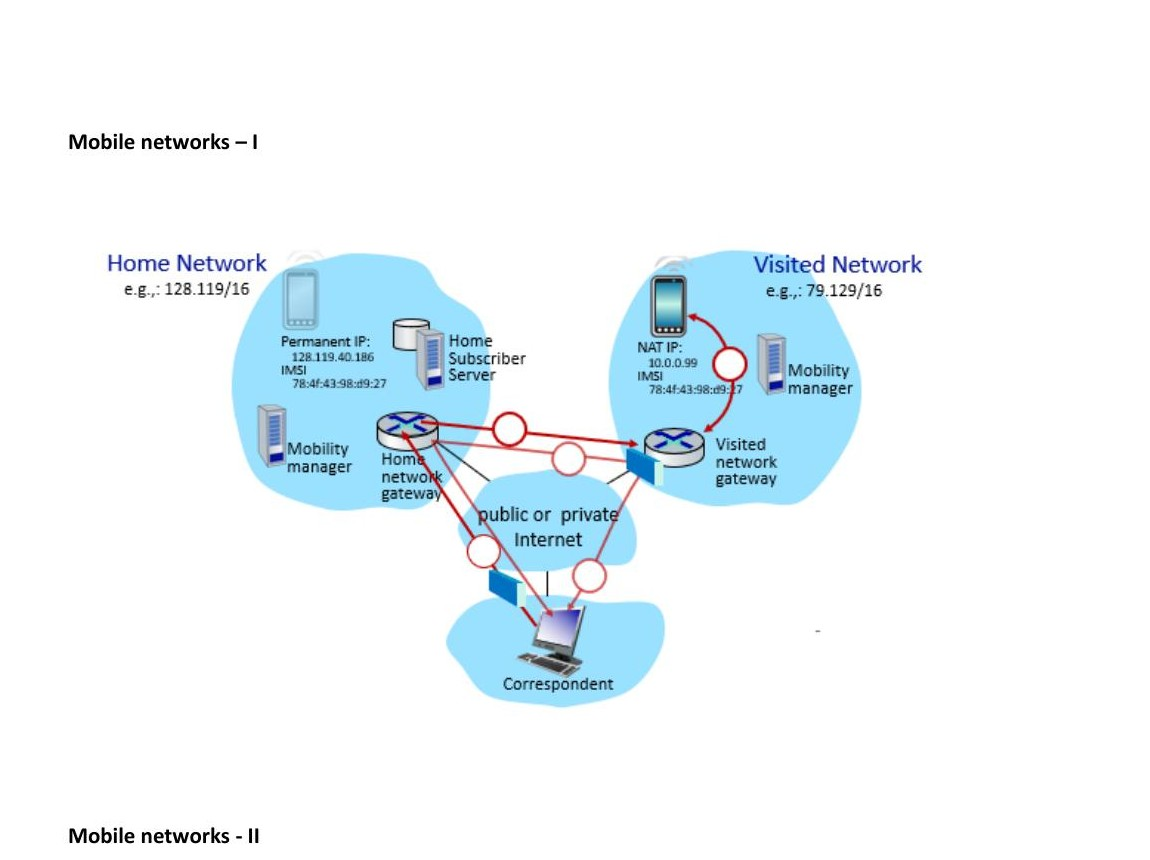
\includegraphics[keepaspectratio]{images/exam-mod2-mobile-networks-I.jpg}}

Nel \textbf{routing indiretto} (o \emph{triangle routing}) --- modalità
standard per le reti 4G LTE e per Mobile IP --- l'idea di base è che
quando il Correspondent vuole inviare dati al dispositivo mobile:

\begin{enumerate}
\def\labelenumi{\arabic{enumi}.}
\tightlist
\item
  Il Correspondent invia il pacchetto all'\textbf{indirizzo permanente}
  del mobile, che appartiene alla home network.
\item
  Il \textbf{Home network gateway} (o P-GW) riceve il pacchetto, lo
  \textbf{incapsula} in un tunnel (tipicamente usando il protocollo GTP
  --- \emph{GPRS Tunneling Protocol}) e lo forwarda al Visited network
  gateway (S-GW/P-GW locale).
\item
  Il \textbf{Visited network gateway} decapsula il pacchetto, applica la
  traduzione \textbf{NAT} (perché il dispositivo ha un IP locale) e lo
  consegna al dispositivo.
\item
  Le risposte del dispositivo possono seguire il percorso inverso oppure
  essere inviate direttamente al Correspondent.
\end{enumerate}

Il percorso forma un \textbf{triangolo}: Correspondent → Home → Visited
→ Mobile, anche se Correspondent e mobile fossero fisicamente vicini.
Questo è il costo dell'approccio, ma il vantaggio è notevole: ogni
cambio di rete visitata è completamente \textbf{trasparente} per il
Correspondent. La nuova rete si registra presso l'HSS e l'endpoint del
tunnel viene aggiornato silenziosamente lato home network, senza che il
Correspondent debba fare nulla.

\begin{calloutnote}{Continuità delle sessioni TCP}

Quando il dispositivo si sposta in una nuova rete visitata, possono
andare persi alcuni datagrammi in transito. Tuttavia le sessioni TCP
rimangono attive: dal punto di vista del corrispondente, la posizione
del mobile è un dettaglio interno alla home network gestito
trasparentemente dal meccanismo di tunneling.

\end{calloutnote}

\section{Routing Diretto}\label{routing-diretto}

\pandocbounded{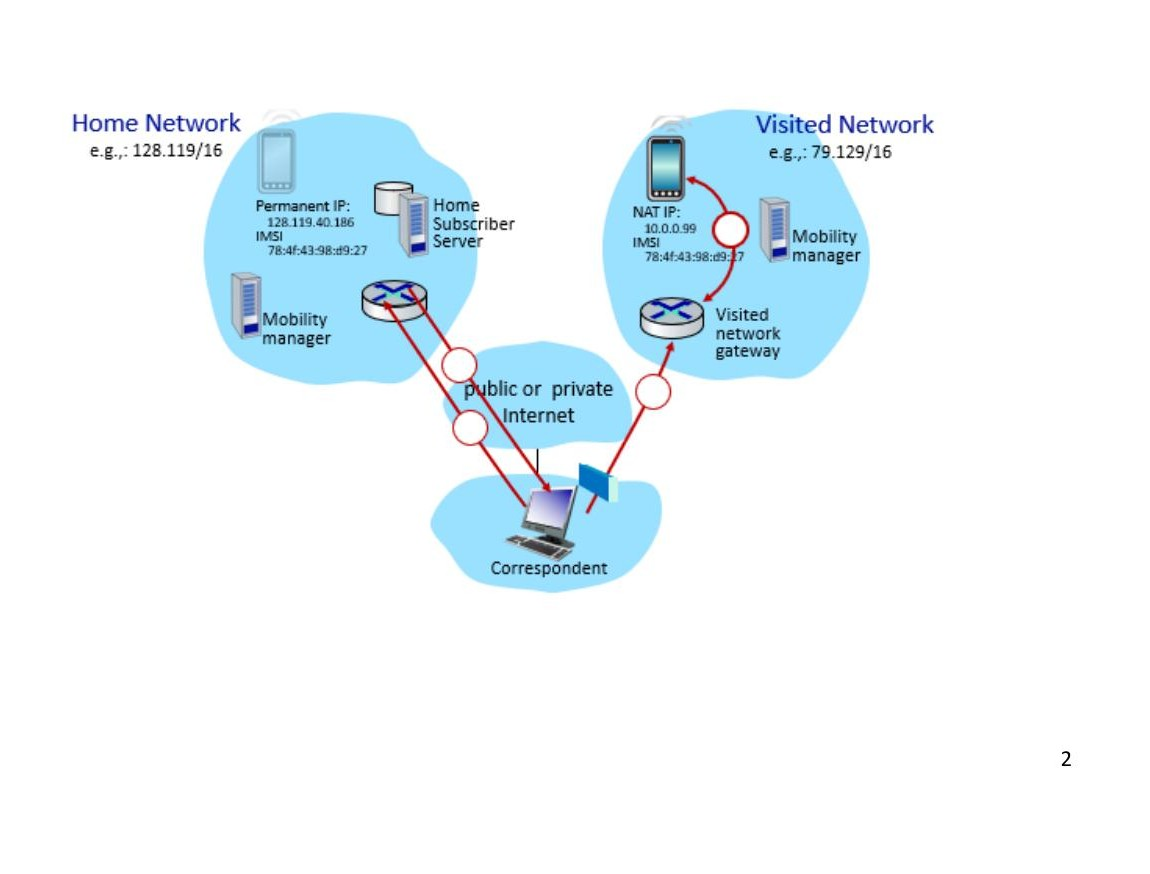
\includegraphics[keepaspectratio]{images/exam-mod2-mobile-networks-II.jpg}}

Nel \textbf{routing diretto}, l'alternativa al triangle routing per le
reti mobili, il Correspondent non invia i pacchetti all'indirizzo
permanente del mobile, ma ottiene prima il suo \textbf{care-of address}
nella rete visitata. La procedura è la seguente:

\begin{enumerate}
\def\labelenumi{\arabic{enumi}.}
\tightlist
\item
  Il Correspondent interroga l'\textbf{HSS} della home network (tramite
  un protocollo apposito) per ottenere l'indirizzo corrente del
  dispositivo mobile nella rete visitata (il care-of address).
\item
  Il Correspondent invia i pacchetti \textbf{direttamente} al care-of
  address nella visited network, bypassando la home network.
\item
  Il Visited network gateway riceve il pacchetto e lo consegna al
  dispositivo mobile.
\end{enumerate}

\textbf{Vantaggi rispetto al routing indiretto:} il percorso è più corto
(nessun triangolo), la latenza è ridotta, e non si sovraccarica
inutilmente la home network.

\textbf{Svantaggi e problemi:} l'approccio \textbf{non è trasparente}
per il Correspondent, che deve eseguire attivamente la query all'HSS.
Inoltre, se il dispositivo cambia rete visitata durante una sessione
attiva, il Correspondent ha interrogato l'HSS \textbf{solo all'inizio
della sessione} e non conosce il nuovo care-of address. Servono quindi
meccanismi aggiuntivi per aggiornare dinamicamente il flusso dati (es.
forwarding dalla vecchia visited network alla nuova, o re-query
dell'HSS), a differenza del routing indiretto dove è sufficiente
cambiare l'endpoint del tunnel.

\begin{callouttip}{Confronto diretto vs indiretto}

{\def\LTcaptype{none} % do not increment counter
\begin{longtable}[]{@{}
  >{\raggedright\arraybackslash}p{(\linewidth - 4\tabcolsep) * \real{0.3333}}
  >{\raggedright\arraybackslash}p{(\linewidth - 4\tabcolsep) * \real{0.3333}}
  >{\raggedright\arraybackslash}p{(\linewidth - 4\tabcolsep) * \real{0.3333}}@{}}
\toprule\noalign{}
\begin{minipage}[b]{\linewidth}\raggedright
Aspetto
\end{minipage} & \begin{minipage}[b]{\linewidth}\raggedright
Routing Indiretto
\end{minipage} & \begin{minipage}[b]{\linewidth}\raggedright
Routing Diretto
\end{minipage} \\
\midrule\noalign{}
\endhead
\bottomrule\noalign{}
\endlastfoot
Percorso pacchetti & Triangolo (via home) & Diretto alla visited \\
Trasparenza per Correspondent & Sì & No (deve interrogare HSS) \\
Gestione cambio rete & Automatica (re-tunnel) & Complessa (deve
aggiornare il Correspondent) \\
Latenza & Maggiore (percorso più lungo) & Minore \\
Adottato in LTE/4G & Sì (per default) & Solo con ottimizzazione
esplicita \\
\end{longtable}
}

\end{callouttip}

\section{L'Architettura Pratica: Mobilità nelle Reti 4G e
Handover}\label{larchitettura-pratica-mobilituxe0-nelle-reti-4g-e-handover}

\pandocbounded{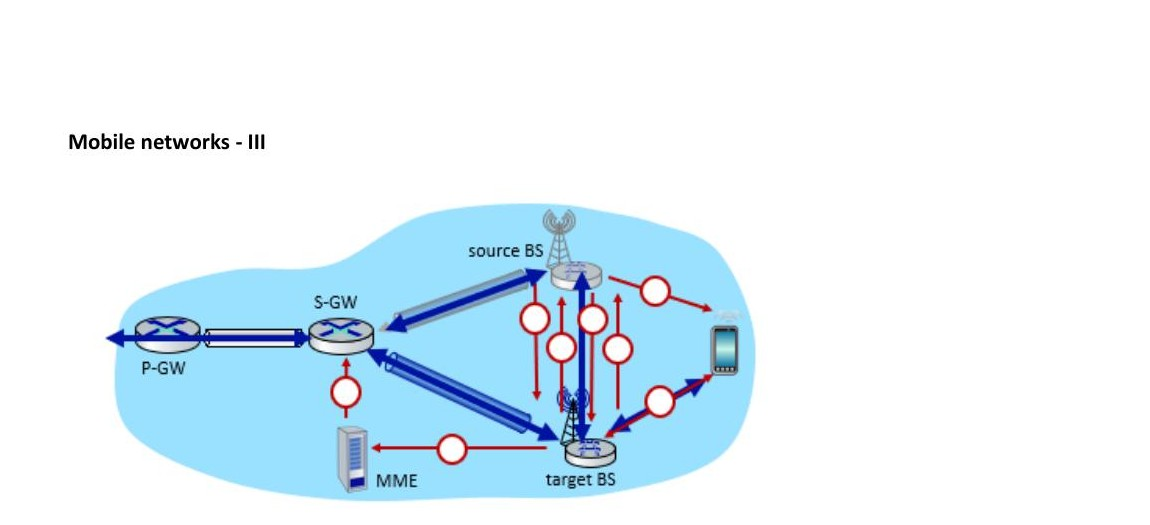
\includegraphics[keepaspectratio]{images/exam-mod2-mobile-networks-III.jpg}}

Quando un dispositivo entra in una rete 4G visitata, la gestione della
mobilità e la transizione tra celle sono gestite tramite un'architettura
ben definita.

\textbf{Architettura del piano dati:} quando il dispositivo è associato
a una BS, il traffico dati fluisce attraverso due tunnel GTP in cascata:
- \textbf{Tunnel BS ↔ S-GW}: connette la Base Station corrente al
Serving Gateway. Quando il dispositivo cambia Base Station, non occorre
ricreare il tunnel --- è sufficiente aggiornare l'indirizzo IP
dell'endpoint sul lato BS. - \textbf{Tunnel S-GW ↔ P-GW}: connette il
Serving Gateway al PDN Gateway (il gateway verso Internet nella home
network), realizzando il routing indiretto.

\textbf{Procedura di handover tra Base Station:} l'handover si attiva
quando il dispositivo si sposta e la qualità del segnale sulla BS
corrente degrada. La procedura completa si articola in sette passi:

\begin{enumerate}
\def\labelenumi{\arabic{enumi}.}
\tightlist
\item
  La \textbf{source BS} rileva il degrado del segnale (o il
  sovraccarico) e decide di avviare l'handover. Sceglie la
  \textbf{target BS} (sulla base delle misure di segnale riportate dal
  dispositivo) e le invia una \textbf{Handover Request}.
\item
  La \textbf{target BS} pre-alloca le risorse radio necessarie e
  risponde con un \textbf{Handover Request ACK} contenente i parametri
  di configurazione per il dispositivo.
\item
  La \textbf{source BS} notifica al dispositivo il cambio imminente; da
  questo momento il dispositivo può già trasmettere tramite la nuova BS
  --- dal punto di vista del dispositivo l'handover è già avvenuto.
\item
  La \textbf{source BS} smette di trasmettere al dispositivo e inizia a
  \textbf{forwardare} i datagrammi in arrivo verso la target BS (che li
  recapita al dispositivo via radio).
\item
  La \textbf{target BS} informa l'\textbf{MME} (\emph{Mobility
  Management Entity}) di essere la nuova BS per il dispositivo.
\item
  L'\textbf{MME} istruisce lo \textbf{S-GW} di aggiornare l'endpoint del
  tunnel dati alla nuova target BS. La source BS riceve conferma e può
  liberare le proprie risorse radio.
\item
  Il traffico fluisce ora attraverso il \textbf{nuovo tunnel} dalla
  target BS allo S-GW, mentre il tunnel S-GW ↔ P-GW rimane invariato.
\end{enumerate}

\begin{callouttip}{Chi decide l’handover?}

È un punto classico da esame: sia la decisione di avviare l'handover sia
la scelta della target BS spettano alla \textbf{source BS} --- non
all'MME. L'MME viene coinvolto solo nella fase finale per aggiornare il
piano dati. Questo riflette la separazione tra control plane (MME
gestisce la mobilità a livello di rete) e data plane (le BS gestiscono
la qualità del segnale radio).

\end{callouttip}

\newpage

\chapter{Software Defined Networking
(SDN)}\label{software-defined-networking-sdn}

Questo paradigma architetturale segna il definitivo passaggio da un
sistema di protocolli puramente distribuiti a un framework di controllo
di rete completamente programmabile.

\begin{calloutdefinition}{Software Defined Networking}

Il \textbf{Software Defined Networking} è un approccio alla gestione
delle reti che sfrutta potenti meccanismi di astrazione per abilitare
configurazioni e operazioni dinamiche ed efficienti a livello
programmatico. La caratteristica distintiva è la separazione netta tra
\textbf{control plane} e \textbf{data plane}.

\end{calloutdefinition}

\begin{center}\rule{0.5\linewidth}{0.5pt}\end{center}

\section{La Separazione tra Data Plane e Control
Plane}\label{la-separazione-tra-data-plane-e-control-plane}

\begin{calloutdefinition}{Data Plane e Control Plane}

Il \textbf{Data Plane (Forwarding)} è l'atto meccanico e istantaneo di
smistare ogni singolo pacchetto in transito su una porta d'uscita del
router. Il \textbf{Control Plane (Routing)} è il processo decisionale,
su scale temporali molto più dilatate, attraverso cui si mappa il
tragitto completo sorgente-destinazione.

\end{calloutdefinition}

Nel tradizionale instradamento IP entrambi coesistono in un modello
\textbf{per-router control plane} fortemente accoppiato: gli algoritmi
risiedono in ogni nodo e calcolano localmente le tabelle di forwarding
in modo decentralizzato. Tale struttura fu ideata per garantire
resilienza, ma rende le moderne operazioni di \emph{Traffic Engineering}
estremamente difficili. I link weight sono l'unico ``manopola di
controllo'' disponibile. Si considerino tre scenari concreti su una rete
con nodi u, v, w, x, y, z:

\begin{callouttip}{Tre scenari impossibili con il routing tradizionale}

\textbf{Scenario 1 --- Percorso specifico}: l'operatore vuole che il
traffico da u a z segua il percorso u→v→w→z anziché il percorso più
breve u→x→y→z. L'unica leva è ridefinire i link weight affinché
l'algoritmo calcoli quella rotta --- ma non esiste garanzia che il
risultato sia quello voluto senza effetti collaterali sugli altri
flussi.

\textbf{Scenario 2 --- Load balancing}: l'operatore vuole dividere il
traffico da u a z equamente tra i due percorsi u→v→w→z e u→x→y→z. Non è
possibile con il routing basato su destinazione: l'algoritmo converge su
un unico percorso minimo.

\textbf{Scenario 3 --- Routing per-flusso}: il nodo w vuole instradare
verso z in modo diverso il traffico blu (proveniente da u) rispetto al
traffico rosso (proveniente da x). Non è possibile con il forwarding
basato sulla sola destinazione (LS, DV): la decisione dipende unicamente
dall'indirizzo di destinazione, non dal flusso.

\end{callouttip}

\begin{center}\rule{0.5\linewidth}{0.5pt}\end{center}

\section{Il Paradigma SDN: Centralizzazione Logica e
Programmabilità}\label{il-paradigma-sdn-centralizzazione-logica-e-programmabilituxe0}

La grande innovazione del SDN è il \textbf{Logically Centralized Control
Plane}: un controller interroga e supervisiona remotamente la topologia
globale calcolando le tabelle di forwarding per tutti i nodi. Mentre nel
modello classico ogni tabella è rigidamente calcolata come
\(T_{i} = SPF(Topology, link\_weights)\) ignorando metriche esterne, nel
modello SDN il controller calcola la funzione globale:

\[
\mathcal{F}: S(t) \rightarrow \{T_1, T_2, \ldots, T_n\}
\]

dove le tabelle di uscita derivano dallo stato \(S(t)\) che ingloba in
tempo reale topologia, traffico totale e vincoli di policy.

\begin{calloutimportant}{Architettura SDN e astrazione Match-Action}

Il SDN poggia su pilastri imprescindibili: una demarcazione netta tra
data plane e control plane; il control plane definisce il comportamento
strategico della rete mentre il data plane applica le direttive ai
pacchetti fisici; l'uso di switch elementari ad alte prestazioni
governati tramite l'astrazione \textbf{match-action} orientata ai flussi
(es. OpenFlow); il ricorso totale a protocolli aperti e programmabili.

\end{calloutimportant}

Il controller SDN comunica su due assi. La \textbf{Southbound API}
(tipicamente OpenFlow) è l'interfaccia verso il basso tra il controller
e gli switch del data plane, tramite cui vengono installate le regole di
forwarding nell'hardware. La \textbf{Northbound API} è l'interfaccia
verso l'alto che dialoga con le applicazioni di gestione (bilanciamento,
routing avanzato, access control), sviluppabili autonomamente da terze
parti indipendentemente dai produttori hardware.

\begin{calloutwarning}{L’illusione del server singolo}

Sebbene logicamente centralizzato, il \emph{SDN Controller} è
fisicamente implementato come un sistema fortemente distribuito. Ciò
assicura tolleranza agli errori, elevata scalabilità e robustezza contro
guasti singoli critici.

\end{calloutwarning}

\begin{center}\rule{0.5\linewidth}{0.5pt}\end{center}

\section{Architettura SDN: I Tre
Componenti}\label{architettura-sdn-i-tre-componenti}

\pandocbounded{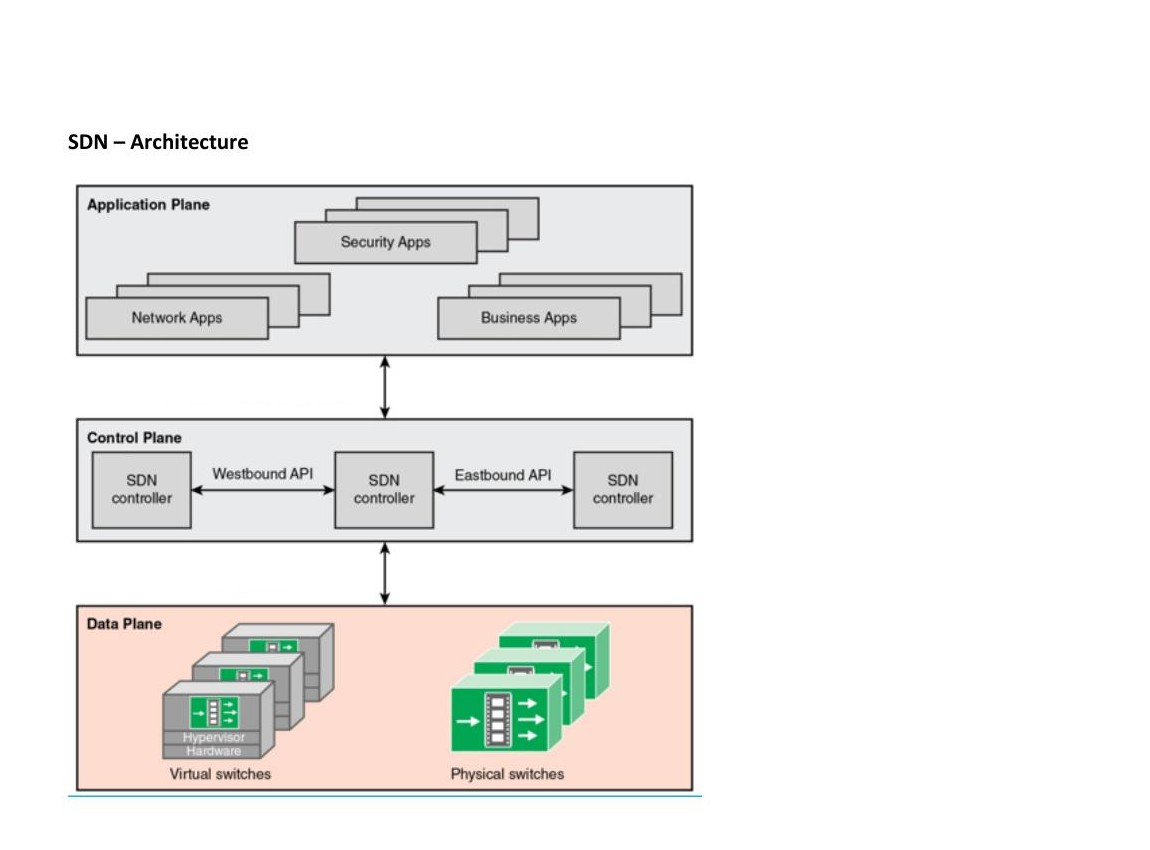
\includegraphics[keepaspectratio]{images/exam-mod2-sdn-architecture.jpg}}

Questo schema illustra l'\textbf{architettura a tre livelli di SDN}, che
realizza la separazione netta tra data plane, control plane e
application plane. L'architettura si articola in tre livelli distinti
con ruoli ben separati:

\subsection{Data-Plane Switches (Livello
inferiore)}\label{data-plane-switches-livello-inferiore}

Contiene gli switch del data plane, che possono essere sia fisici
(hardware commodity a basso costo) sia virtuali (Open vSwitch su
hypervisor). Sono dispositivi semplici e veloci: il loro unico compito è
applicare meccanicamente le regole di forwarding (match-action) ai
pacchetti in transito secondo le flow table installate dal controller.
Non calcolano nulla autonomamente. Le flow table vengono calcolate e
installate da remoto dal controller, non localmente. Lo switch espone
un'API standardizzata (tipicamente OpenFlow) che definisce cosa è
controllabile dall'esterno e cosa no, e un protocollo per comunicare con
il controller.

\subsection{SDN Controller / Control Plane (Livello
centrale)}\label{sdn-controller-control-plane-livello-centrale}

Il controller SDN svolge il ruolo di \textbf{sistema operativo di rete}:
mantiene una visione aggiornata dello stato globale della rete
(topologia, link attivi, tabelle di forwarding). È il punto di
mediazione tra le applicazioni che esprimono policy di alto livello e
gli switch che le devono applicare. Contiene il controller SDN, o meglio
una \textbf{rete di controller SDN} distribuiti. Sebbene appaia come
un'entità logicamente centralizzata (ha una visione globale della rete),
è implementato fisicamente come sistema distribuito per garantire
performance, scalabilità, tolleranza ai guasti e robustezza. Il
controller mantiene: la topologia della rete, le statistiche dei flussi,
i link attivi, le tabelle di forwarding. Comunica verso il basso con il
Data Plane tramite la \textbf{Southbound API} (tipicamente OpenFlow), e
verso l'alto con le applicazioni tramite la \textbf{Northbound API}. I
controller comunicano tra loro tramite \textbf{Westbound/Eastbound API}
per sincronizzare lo stato globale.

\subsection{Network-Control Applications / Application Plane (Livello
superiore)}\label{network-control-applications-application-plane-livello-superiore}

Le applicazioni di controllo (\emph{network-control applications}) sono
il vero ``cervello'' della rete: implementano le funzioni di controllo
(routing, access control, load balancing, monitoraggio, rilevamento
anomalie, \ldots) sfruttando i servizi e le API esposte dal controller.
Il punto chiave è che sono \textbf{unbundled}: possono essere sviluppate
e fornite da terze parti indipendentemente dai produttori hardware e
software del controller. Questo disaccoppiamento abilita un ecosistema
aperto in cui l'innovazione a livello applicativo è indipendente
dall'hardware sottostante. Le applicazioni esprimono policy di alto
livello al controller tramite la Northbound API.

\begin{calloutnote}{Il valore dell’architettura a livelli}

La separazione in tre piani replica il principio dei livelli di
astrazione di Internet. Ogni livello si può evolvere indipendentemente:
nuovi algoritmi di routing nel Control Plane, nuove applicazioni
nell'Application Plane, nuovo hardware nel Data Plane --- senza impatto
sugli altri livelli. Questo è il vantaggio principale rispetto alle reti
tradizionali con logica chiusa nell'hardware proprietario.

\end{calloutnote}

\newpage

\chapter{Software Defined Networking (SDN) ---
Architettura}\label{software-defined-networking-sdn-architettura}

Il Software Defined Networking è un paradigma architetturale che separa
nettamente il \textbf{piano di controllo} (\emph{control plane}) dal
\textbf{piano dati} (\emph{data plane}). Questa separazione permette di
programmare il comportamento della rete in modo centralizzato,
eliminando la rigidità dei dispositivi di rete tradizionali che
incorporano sia la logica di instradamento che la funzione di
forwarding.

\section{Il Paradigma SDN e la Separazione dei
Piani}\label{il-paradigma-sdn-e-la-separazione-dei-piani}

Le funzioni di rete a livello network si dividono in due categorie
temporalmente molto diverse: il \textbf{forwarding} (spostare pacchetti
dall'input all'output appropriato) avviene su scala temporale dei
pacchetti (\emph{fast timescales}), mentre il \textbf{routing}
(determinare il percorso dei pacchetti da sorgente a destinazione)
avviene su scala degli eventi di controllo (\emph{slow timescales}). In
una rete tradizionale, queste due funzioni sono tightly coupled nello
stesso dispositivo.

\subsection{Esempio di rete gestita con
SDN}\label{esempio-di-rete-gestita-con-sdn}

\pandocbounded{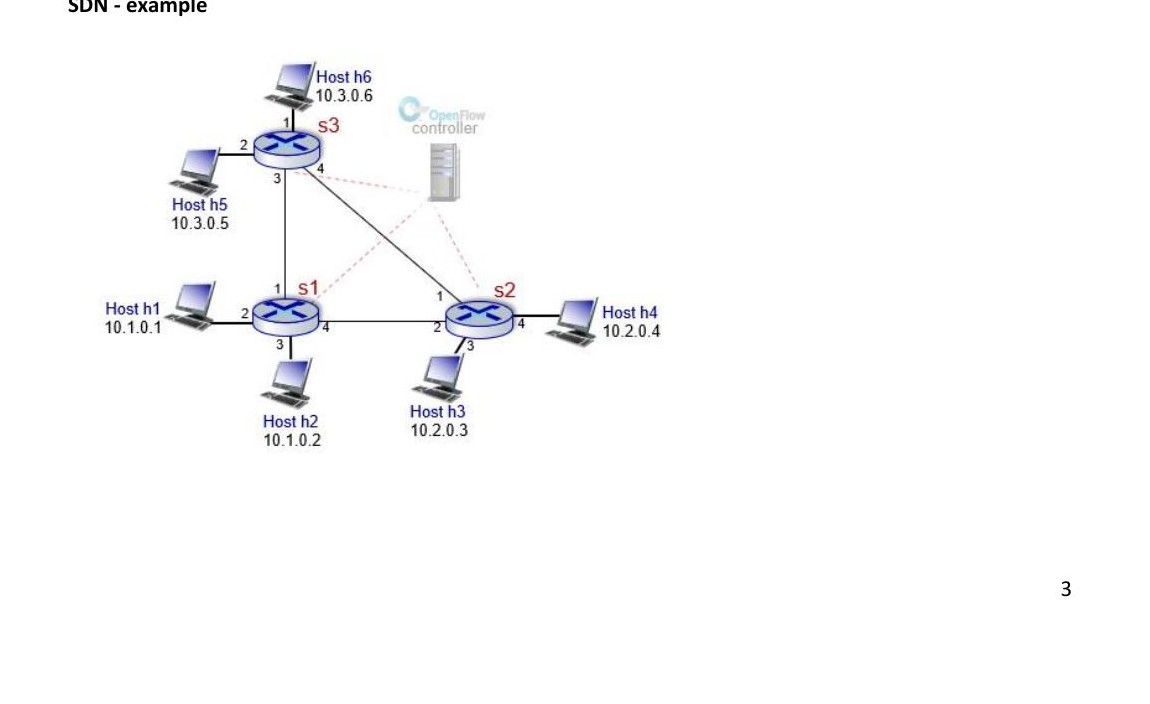
\includegraphics[keepaspectratio]{images/exam-mod2-sdn-example.jpg}}

Questo schema è un esempio concreto di rete gestita con SDN per mostrare
come il \textbf{control plane centralizzato} possa implementare
politiche impossibili con il routing tradizionale.

Nell'architettura mostrata, il \textbf{controller OpenFlow} mantiene una
visione globale della topologia: conosce tutti gli switch, tutte le loro
porte, e dove si trovano i vari host. Le flow table degli switch s1, s2,
s3 vengono popolate \textbf{dal controller}, non calcolate localmente
dagli switch.

\textbf{Traffic Engineering con SDN:} supponiamo che il controller
voglia bilanciare il traffico da h1 (10.1.0.1) verso h4 (10.2.0.4) su
due percorsi: - Percorso A: h1 → s1 → s2 → h4 - Percorso B: h1 → s1 → s3
→ s2 → h4

Con il routing IP tradizionale questo è impossibile: l'algoritmo SPF
converge su un solo percorso minimo. Con SDN, il controller installa
regole diverse in s1 per flussi diversi (es. dividendo per porta
sorgente TCP), realizzando il load balancing.

\textbf{Forwarding basato su flusso:} il controller può distinguere il
traffico h1→h4 dal traffico h2→h4 e applicare politiche diverse. Ad
esempio: - Traffico h1→h4: percorso s1→s2, priorità alta - Traffico
h2→h4: percorso s1→s3→s2, priorità normale

Questo è il \textbf{routing per-flusso}, impossibile nel routing
tradizionale destination-based.

\textbf{Topology discovery:} il controller scopre la topologia inviando
pacchetti LLDP (\emph{Link Layer Discovery Protocol}) tramite gli
switch. Ogni switch incapsula un pacchetto LLDP e lo invia su tutte le
porte; quando un altro switch lo riceve, lo invia al controller, che
così ricostruisce le connessioni tra switch.

\begin{center}\rule{0.5\linewidth}{0.5pt}\end{center}

\section{Architettura SDN a Tre
Livelli}\label{architettura-sdn-a-tre-livelli}

\pandocbounded{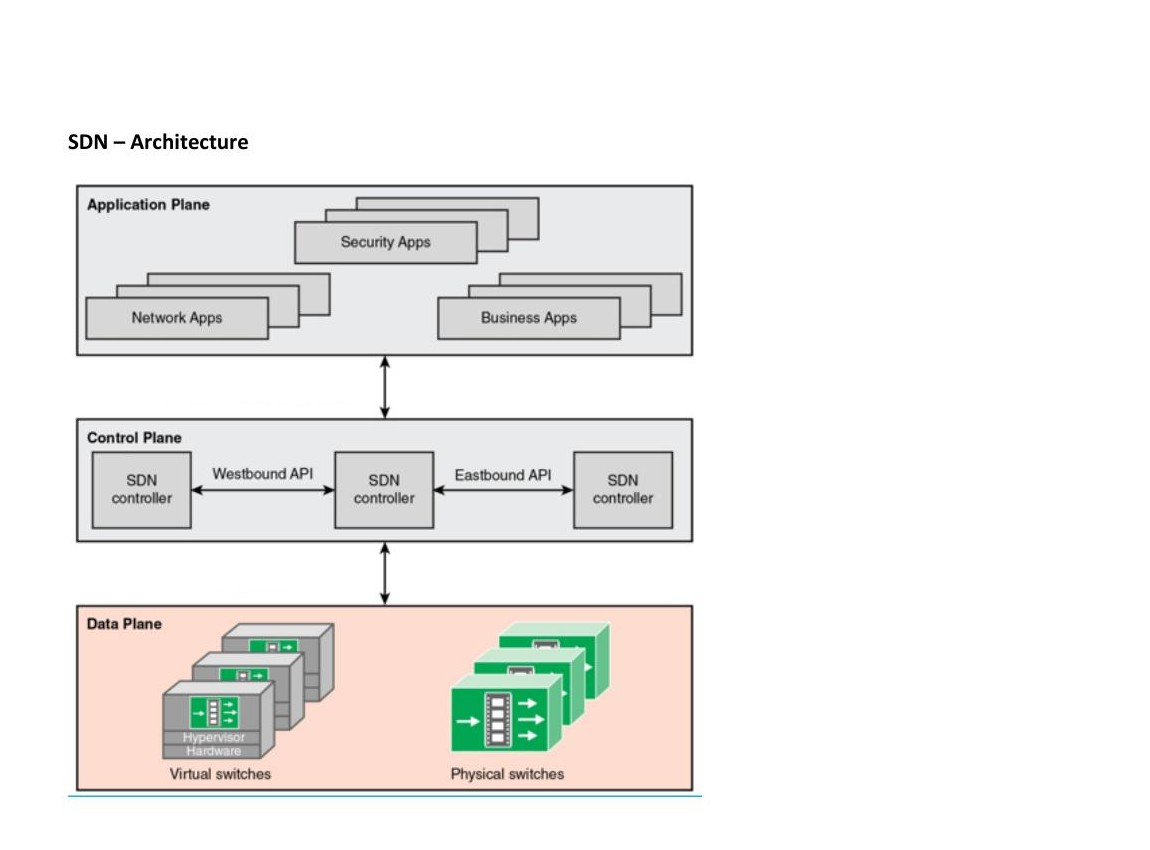
\includegraphics[keepaspectratio]{images/exam-mod2-sdn-architecture.jpg}}

L'architettura SDN è organizzata in tre livelli che realizza la
separazione netta tra data plane, control plane e application plane.

\textbf{Data Plane (Livello inferiore):} contiene gli switch del data
plane, che possono essere sia fisici (hardware commodity a basso costo)
sia virtuali (Open vSwitch su hypervisor). Sono dispositivi semplici: il
loro unico compito è applicare meccanicamente le regole di forwarding
(match-action) ai pacchetti in transito secondo le flow table installate
dal controller. Non calcolano nulla autonomamente. L'API per il
controllo (es. OpenFlow) definisce cosa è controllabile e cosa non lo è.

\textbf{Control Plane (Livello centrale):} contiene il controller SDN, o
meglio una \textbf{rete di controller SDN} distribuiti (\emph{network
operating system}). Sebbene appaia come un'entità logicamente
centralizzata (ha una visione globale della rete), è implementato
fisicamente come sistema distribuito per garantire tolleranza ai guasti
e scalabilità. Il controller mantiene: la topologia della rete, le
statistiche dei flussi, i link attivi, le tabelle di forwarding.
Comunica verso il basso con il Data Plane tramite la \textbf{Southbound
API} (tipicamente OpenFlow), e verso l'alto con le applicazioni tramite
la \textbf{Northbound API}. I controller comunicano tra loro tramite
\textbf{Westbound/Eastbound API} per sincronizzare lo stato globale.

\textbf{Application Plane (Livello superiore):} contiene le applicazioni
di controllo della rete (\emph{network-control applications}), il vero
``cervello'' del sistema. Sono \textbf{unbundled}: possono essere
sviluppate da terze parti indipendentemente dai produttori hardware e
software del controller. Esempi: load balancer, firewall, traffic
engineering, monitoraggio, rilevamento anomalie. Le applicazioni
esprimono policy di alto livello al controller tramite la Northbound
API.

\begin{center}\rule{0.5\linewidth}{0.5pt}\end{center}

\section{SDN Data Plane}\label{sdn-data-plane}

Il data plane è composto da dispositivi di forwarding --- switch fisici
e virtuali --- che trasportano e processano i dati secondo le decisioni
del control plane.

\subsection{Forwarding Generalizzato e
Match-Action}\label{forwarding-generalizzato-e-match-action}

\pandocbounded{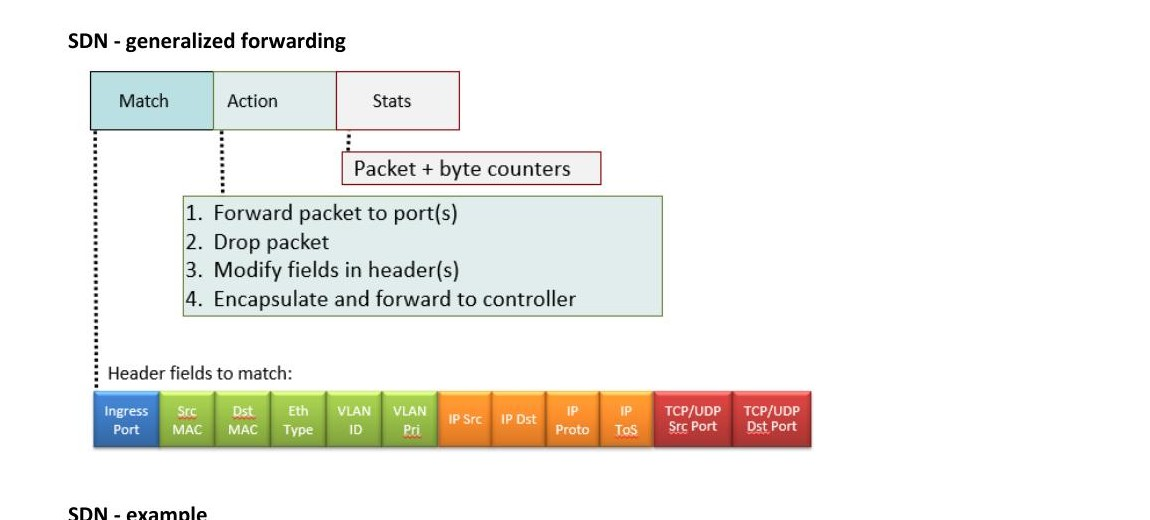
\includegraphics[keepaspectratio]{images/exam-mod2-sdn-generalized-forwarding.jpg}}

Questo schema illustra il concetto di \textbf{forwarding generalizzato}
(\emph{generalized forwarding}) in SDN, che è l'astrazione fondamentale
che rende il data plane programmabile.

Nell'approccio tradizionale, i router inoltrano i pacchetti basandosi
\textbf{solo sull'indirizzo IP di destinazione} (\emph{destination-based
forwarding}). OpenFlow generalizza questo concetto con l'astrazione
\textbf{match-action}: ogni pacchetto viene confrontato con le regole
nella flow table, e quando c'è un match, viene eseguita l'azione
corrispondente.

\textbf{I campi di match} possono essere qualsiasi combinazione dei
seguenti: - Livello 1: \textbf{Ingress Port} (la porta fisica da cui è
arrivato il pacchetto) - Livello 2 (Datalink): Src MAC, Dst MAC, Eth
Type, VLAN ID, VLAN Priority - Livello 3 (Rete): IP Src, IP Dst, IP
Protocol, IP ToS - Livello 4 (Trasporto): TCP/UDP Src Port, TCP/UDP Dst
Port

Questo consente di distinguere flussi in base a qualsiasi combinazione
di questi campi: non solo la destinazione IP, ma anche il protocollo, le
porte, le VLAN, ecc. Si parla di \textbf{flow-based forwarding}.

\textbf{Le azioni possibili} sono: 1. \textbf{Forward to port(s)}: invia
il pacchetto su una o più porte (forwarding normale, broadcast,
multicast). 2. \textbf{Drop}: scarta il pacchetto (firewall, access
control). 3. \textbf{Modify fields in header}: modifica campi
dell'intestazione prima di forwardare (NAT, QoS marking, VLAN tagging).
4. \textbf{Encapsulate and forward to controller}: invia il pacchetto al
controller SDN per una decisione centralizzata (usato per pacchetti non
matchati da nessuna regola --- \emph{table-miss}).

\textbf{Stats}: ogni entry mantiene contatori di pacchetti e byte, utili
per monitoring e traffic engineering.

\begin{callouttip}{Generalità del match-action}

L'astrazione match-action è sufficientemente generale da esprimere:
routing IP (match su IP dst), load balancing (match su src/dst + hash),
firewall (match su src/dst/protocol + drop), NAT (match + modify). Un
singolo modello unifica dispositivi che nelle reti tradizionali
richiederebbero apparati separati.

\end{callouttip}

\begin{center}\rule{0.5\linewidth}{0.5pt}\end{center}

\subsection{OpenFlow Switch e Flow Table
Pipeline}\label{openflow-switch-e-flow-table-pipeline}

\pandocbounded{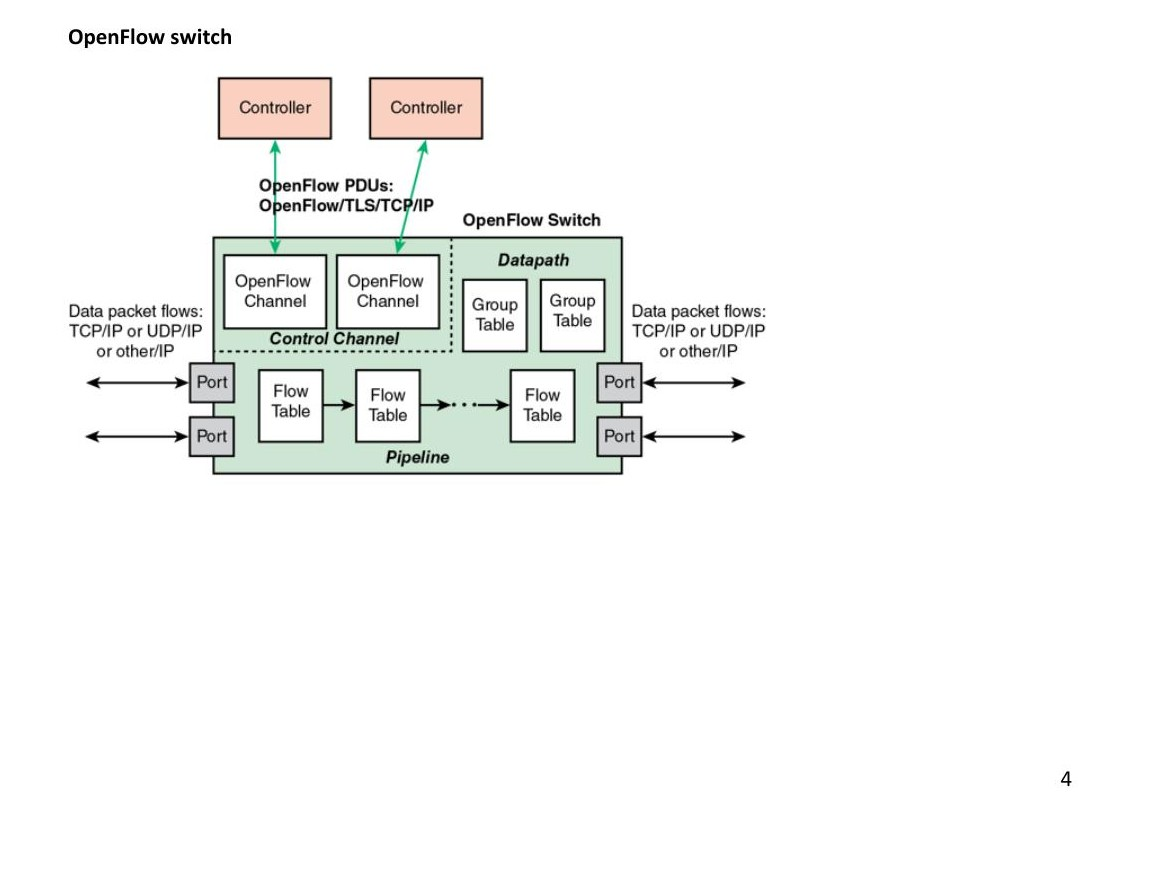
\includegraphics[keepaspectratio]{images/exam-mod2-openflow-switch.jpg}}

Lo schema illustra l'architettura interna di uno switch OpenFlow,
distinguendo il \textbf{piano dati interno} (\emph{Datapath}) dal
\textbf{canale di controllo} (\emph{Control Channel}).

\textbf{Ports:} lo switch ha porte fisiche su cui arrivano e partono i
data packet flow (TCP/IP, UDP/IP, altri). Sono le interfacce verso la
rete esterna.

\textbf{Pipeline di Flow Table:} quando un pacchetto entra in una porta,
viene processato attraverso una catena (\emph{pipeline}) di Flow Table
in sequenza, dalla tabella 0 in poi. In ogni tabella si cerca un match
con le regole installate dal controller: - Se c'è un match → si esegue
l'azione (forward, drop, modify, ecc.) e si passa alla tabella
successiva o si finalizza. - Se non c'è match → si applica la regola di
\emph{table-miss} (tipicamente: invia al controller per una decisione).

\textbf{Group Tables:} le Group Tables consentono azioni più complesse
che non si possono esprimere con le semplici Flow Table: ad esempio la
replica di un pacchetto su più porte (multicast/broadcast), il
fast-failover (selezionare automaticamente una porta alternativa se
quella principale è down), o il load balancing su un gruppo di porte.

\textbf{Control Channel:} è il canale sicuro (tipicamente TLS su TCP)
attraverso cui lo switch OpenFlow comunica con il controller. Il canale
usa il \textbf{protocollo OpenFlow} per scambiarsi tre tipi di messaggi:
- \textbf{Controller → Switch}: \emph{Flow-Mod}
(installa/modifica/cancella una flow entry), \emph{Packet-Out} (invia un
pacchetto da una porta specifica), \emph{Stats-Request}. -
\textbf{Switch → Controller}: \emph{Packet-In} (invia un pacchetto al
controller quando non c'è match), \emph{Flow-Removed} (notifica la
scadenza di una entry), \emph{Port-Status}, \emph{Stats-Reply}. -
\textbf{Bidirezionali}: \emph{Hello} (handshake iniziale), \emph{Echo
Request/Reply} (keepalive).

\begin{calloutnote}{Multi-controller}

Uno switch OpenFlow può connettersi a più controller per ridondanza: uno
è il controller primario, gli altri sono di backup. Se il controller
primario va offline, il backup prende il controllo senza interruzione
del servizio.

\end{calloutnote}

\begin{center}\rule{0.5\linewidth}{0.5pt}\end{center}

\section{SDN Control Plane e Interazione con il Data
Plane}\label{sdn-control-plane-e-interazione-con-il-data-plane}

\pandocbounded{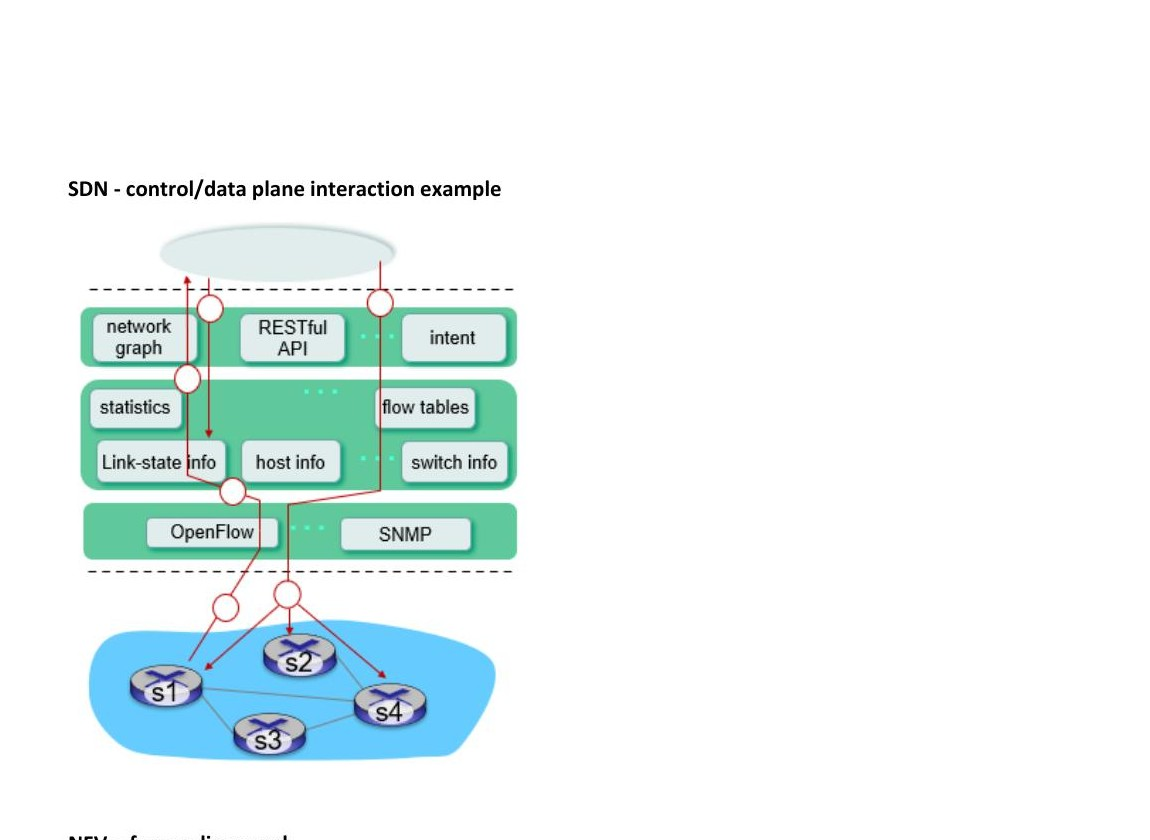
\includegraphics[keepaspectratio]{images/exam-mod2-sdn-control-data-interaction.jpg}}

Questo schema mostra come il controller SDN interagisce concretamente
con il data plane, evidenziando le due direzioni di comunicazione:
\textbf{southbound} (controller → switch) e \textbf{northbound} (switch
→ controller).

\textbf{Il controller SDN mantiene internamente:} - \textbf{Network
graph}: un grafo della topologia completo, aggiornato in tempo reale.
Ogni nodo è uno switch o un host, ogni arco è un link con la sua
capacità. - \textbf{Link-state info}: lo stato di ogni link
(attivo/down, latenza, utilizzo) raccolto tramite LLDP o SNMP. -
\textbf{Host info}: la posizione di ogni host nella rete (a quale porta
di quale switch è connesso). - \textbf{Switch info}: le caratteristiche
di ogni switch (numero di porte, OpenFlow version, capabilities). -
\textbf{Statistics}: contatori di pacchetti e byte per ogni flow entry,
per traffic engineering e monitoring. - \textbf{Flow tables}: le regole
di forwarding da installare negli switch.

\textbf{Interfaccia verso le applicazioni (Northbound):} -
\textbf{RESTful API}: le applicazioni di rete (routing, load balancing,
ACL) interrogano e modificano lo stato del controller tramite API REST.
- \textbf{Intent}: alcune implementazioni supportano un livello di
astrazione più alto, dove le applicazioni esprimono ``intenzioni'' (es.
``garantisci 10 Mbps di banda tra h1 e h2'') che il controller traduce
in flow rules.

\textbf{Interfaccia verso gli switch (Southbound):} - \textbf{OpenFlow}:
protocollo principale per installare le flow rule e ricevere packet-in
dagli switch. - \textbf{SNMP} (\emph{Simple Network Management
Protocol}): usato per raccogliere statistiche di gestione dagli switch
(link status, error counters, ecc.) anche da switch non necessariamente
OpenFlow.

\subsection{Topology Discovery con
LLDP}\label{topology-discovery-con-lldp}

La topology discovery in reti OpenFlow si basa sul \textbf{Link Layer
Discovery Protocol (LLDP)}, standardizzato da IEEE nel 2005 e 2009.

Il processo si svolge in quattro passi: 1. Il controller genera un
\textbf{Packet-Out} per ogni porta attiva su ogni switch scoperto,
incapsulando al suo interno un frame LLDP con il Chassis ID e il Port ID
dello switch sorgente. 2. Quando uno switch OF riceve un messaggio
Packet-Out con un frame LLDP, lo \textbf{forwarda} sulla porta
specificata nel Port ID verso lo switch adiacente. 3. Lo switch
adiacente, ricevendo il frame LLDP su una porta non di controllo, lo
\textbf{incapsula in un Packet-In} indirizzato al controller, includendo
i propri Switch ID e Port ID come metadata. 4. Il controller riceve il
Packet-In ed \textbf{estrae le informazioni}: conosce ora lo Switch ID e
Port ID del frame LLDP (mittente originale) e lo Switch ID e Port ID del
Packet-In (ricevente). Da questi dati deduce che esiste un link tra quei
due switch su quelle specifiche porte.

\newpage

\chapter{Network Function
Virtualization}\label{network-function-virtualization}

La \textbf{Network Function Virtualization} (NFV) rappresenta uno dei
cambiamenti di paradigma più significativi nell'ingegneria delle reti
degli ultimi anni. L'idea fondamentale è semplice ma rivoluzionaria:
spostare le funzioni di rete --- firewall, bilanciatori di carico,
gateway --- dall'hardware proprietario dedicato a software eseguito su
infrastruttura virtualizzata generica.

\begin{center}\rule{0.5\linewidth}{0.5pt}\end{center}

\section{NFV: l'idea fondamentale}\label{nfv-lidea-fondamentale}

\subsection{Decoupling tra funzioni e
hardware}\label{decoupling-tra-funzioni-e-hardware}

Il principio cardine di NFV è il \textbf{disaccoppiamento}
(\emph{decoupling}) tra le funzioni di rete e l'hardware su cui girano.
Le funzioni non sono più implementate in appliance fisiche dedicate, ma
come \textbf{software} eseguito su infrastruttura virtualizzata standard
(macchine virtuali o container su server COTS --- \emph{Commercial
Off-The-Shelf}).

\begin{calloutdefinition}{VNF — Virtualized Network Function}

Una \textbf{Virtualized Network Function} (VNF) è l'implementazione
software di una funzione di rete tradizionalmente realizzata in hardware
dedicato (firewall, load balancer, NAT, ecc.), eseguita su risorse
virtualizzate (VM o container).

\end{calloutdefinition}

\begin{center}\rule{0.5\linewidth}{0.5pt}\end{center}

\section{NFV --- Forwarding Graph}\label{nfv-forwarding-graph}

\pandocbounded{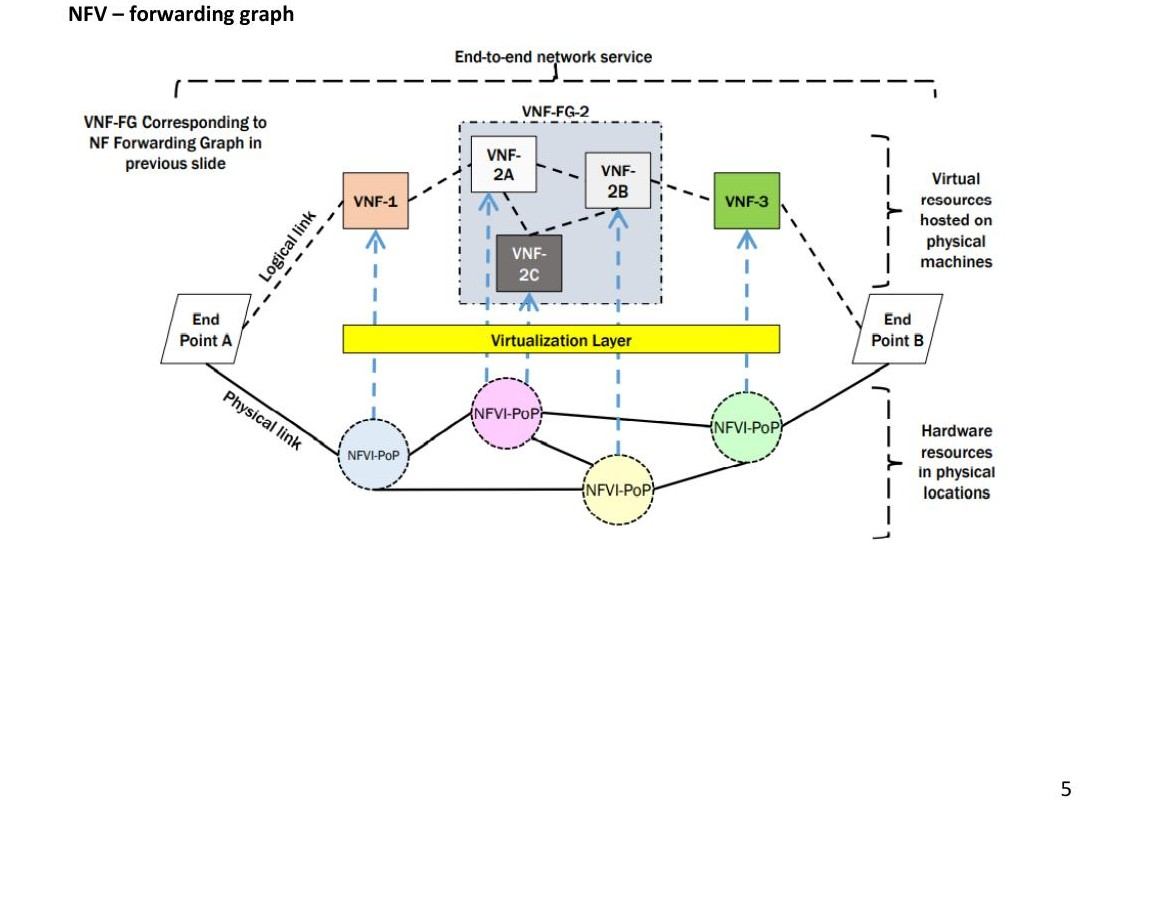
\includegraphics[keepaspectratio]{images/exam-mod2-nfv-forwarding-graph.jpg}}

Questo schema rappresenta il concetto di \textbf{VNF Forwarding Graph}
(VNF-FG), che è il modo in cui NFV formalizza un servizio di rete
end-to-end.

\textbf{L'idea fondamentale di NFV:} invece di implementare funzioni di
rete (firewall, NAT, load balancer, media gateway) in hardware
proprietario dedicato, NFV le implementa come software --- chiamate
\textbf{VNF} (\emph{Virtualized Network Functions}) --- eseguito su
infrastruttura hardware commodity (server COTS). Il decoupling tra
funzione e hardware porta flessibilità, scalabilità e riduzione dei
costi.

\textbf{Il Forwarding Graph:} un servizio di rete non è una singola
funzione, ma una \textbf{composizione di funzioni} applicate in sequenza
al traffico. Il grafo mostra: - Il traffico entra da \textbf{End Point
A}, passa attraverso \textbf{VNF-1}, poi attraverso il sotto-grafo
\textbf{VNF-FG-2} (che a sua volta compone internamente VNF-2A → VNF-2B
e VNF-2C in parallelo), poi attraverso \textbf{VNF-3}, e infine
raggiunge \textbf{End Point B}. - I link logici (tratteggiati)
rappresentano connettività virtuale: due VNF sono logicamente connesse,
ma possono fisicamente trovarsi su macchine diverse.

\textbf{I grafi sono nidificati:} VNF-FG-2 è esso stesso un sotto-grafo
all'interno del grafo principale. Questo consente la riusabilità:
VNF-FG-2 può essere istanziato in altri servizi senza ridefinirlo.

\textbf{L'infrastruttura fisica (NFVI):} le VNF girano su nodi fisici
chiamati \textbf{NFVI-PoP} (\emph{Network Function Virtualization
Infrastructure Point of Presence}). Sono server COTS distribuiti
geograficamente, interconnessi da una rete di trasporto fisica. La
\textbf{Virtualization Layer} (hypervisor o container engine) astrae le
risorse fisiche e consente a più VNF di condividere lo stesso hardware.

\textbf{Il problema del VNF placement:} dato il grafo logico del
servizio, occorre decidere dove deployare fisicamente ogni VNF
nell'infrastruttura. Questo è un problema di ottimizzazione NP-hard che
considera: latenza end-to-end, capacità dei nodi, banda dei link, costi
di deployment, requisiti di QoS per ogni slice di rete.

\begin{center}\rule{0.5\linewidth}{0.5pt}\end{center}

\section{NFV --- Management and
Orchestration}\label{nfv-management-and-orchestration}

\pandocbounded{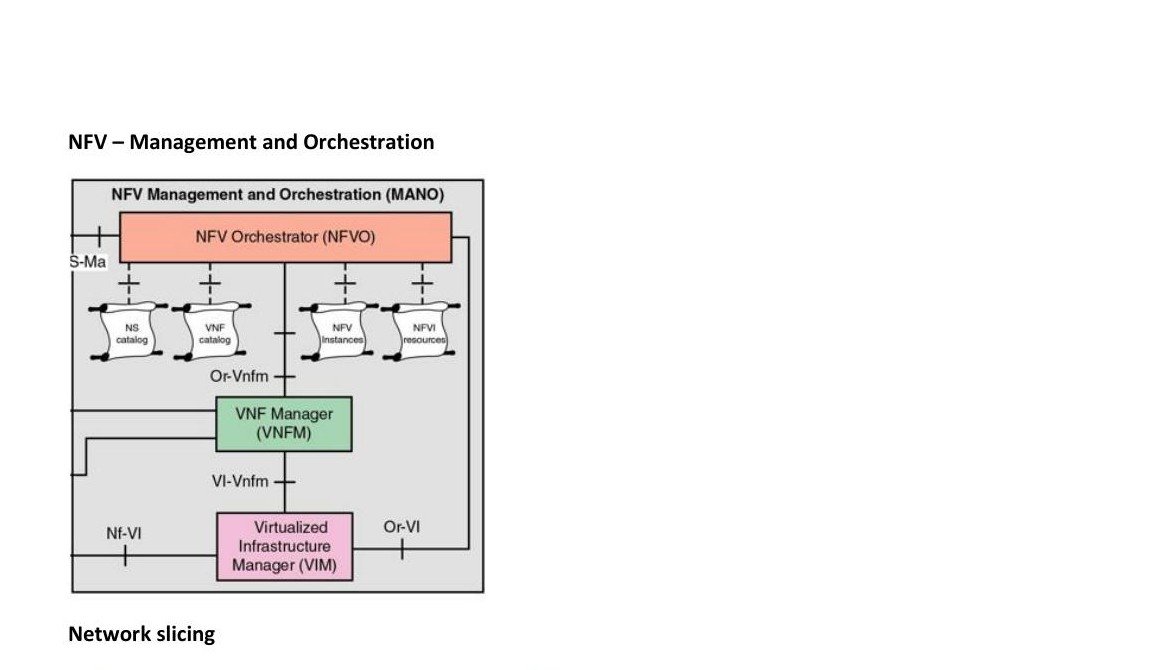
\includegraphics[keepaspectratio]{images/exam-mod2-nfv-mano.jpg}}

Questo schema mostra il framework di \textbf{gestione e orchestrazione
NFV} standardizzato da ETSI, che è il ``piano di controllo''
dell'ecosistema NFV.

\textbf{NFV Orchestrator (NFVO):} è il componente di più alto livello.
Ha due responsabilità principali: 1. \textbf{Network services
orchestration}: gestisce il ciclo di vita dei \textbf{Network Service
(NS)} end-to-end, ovvero istanzia, aggiorna e termina l'intero VNF
Forwarding Graph. Può istanziare nuovi VNFM se necessario. 2.
\textbf{Resource orchestration}: gestisce le risorse globali dell'NFVI,
allocandole ai servizi in base alle policy e ai requisiti di QoS. Il
NFVO mantiene due repository: il \textbf{NS Catalog} (template dei
servizi di rete come Network Service Descriptor) e il \textbf{VNF
Catalog} (descrittori di ogni VNF, i VNFD).

\textbf{VNF Manager (VNFM):} gestisce il \textbf{ciclo di vita delle
istanze VNF} singole: - \textbf{Istanziazione}: crea una nuova istanza
VNF su una VM o container nell'NFVI. - \textbf{Scaling}: aumenta o
riduce la capacità di una VNF (scaling out/in orizzontale, scaling
up/down verticale) in base al carico. - \textbf{Healing}: rileva e
gestisce i fault delle VNF (auto-healing o assistito). -
\textbf{Terminazione}: distrugge l'istanza quando non serve più. Il VNFM
comunica con il NFVO tramite \textbf{Or-Vnfm} e con il VIM tramite
\textbf{Vi-Vnfm} (o \textbf{Ve-Vnfm} verso le VNF stesse).

\textbf{Virtualized Infrastructure Manager (VIM):} controlla e gestisce
le risorse fisiche e virtuali dell'NFVI (compute, storage, network).
Piattaforme IaaS come \textbf{OpenStack} fungono da VIM. Il VIM alloca
VM o container alle VNF, configura la rete virtuale (vSwitch, VLAN), e
monitora l'utilizzo delle risorse. Un MANO può orchestrare più VIM
distribuiti geograficamente.

\textbf{Le interfacce di riferimento:} - \textbf{Or-Vi} (NFVO → VIM):
l'orchestratore può richiedere risorse direttamente al VIM. -
\textbf{S-Ma}: collega sistemi OSS/BSS dell'operatore (Operations
Support System / Business Support System) al MANO per l'integrazione con
i sistemi aziendali.

\begin{calloutnote}{Implementazioni open source}

Le principali implementazioni open source del MANO sono \textbf{OSM}
(\emph{Open Source MANO}, promossa da ETSI) e \textbf{ONAP} (\emph{Open
Network Automation Platform}, Linux Foundation). Entrambe sono usate
nelle reti 5G commerciali.

\end{calloutnote}

\newpage

\chapter{Teoria dei Segnali: Serie di
Fourier}\label{teoria-dei-segnali-serie-di-fourier}

\section{Serie di Fourier: dal Tempo alla
Frequenza}\label{serie-di-fourier-dal-tempo-alla-frequenza}

\pandocbounded{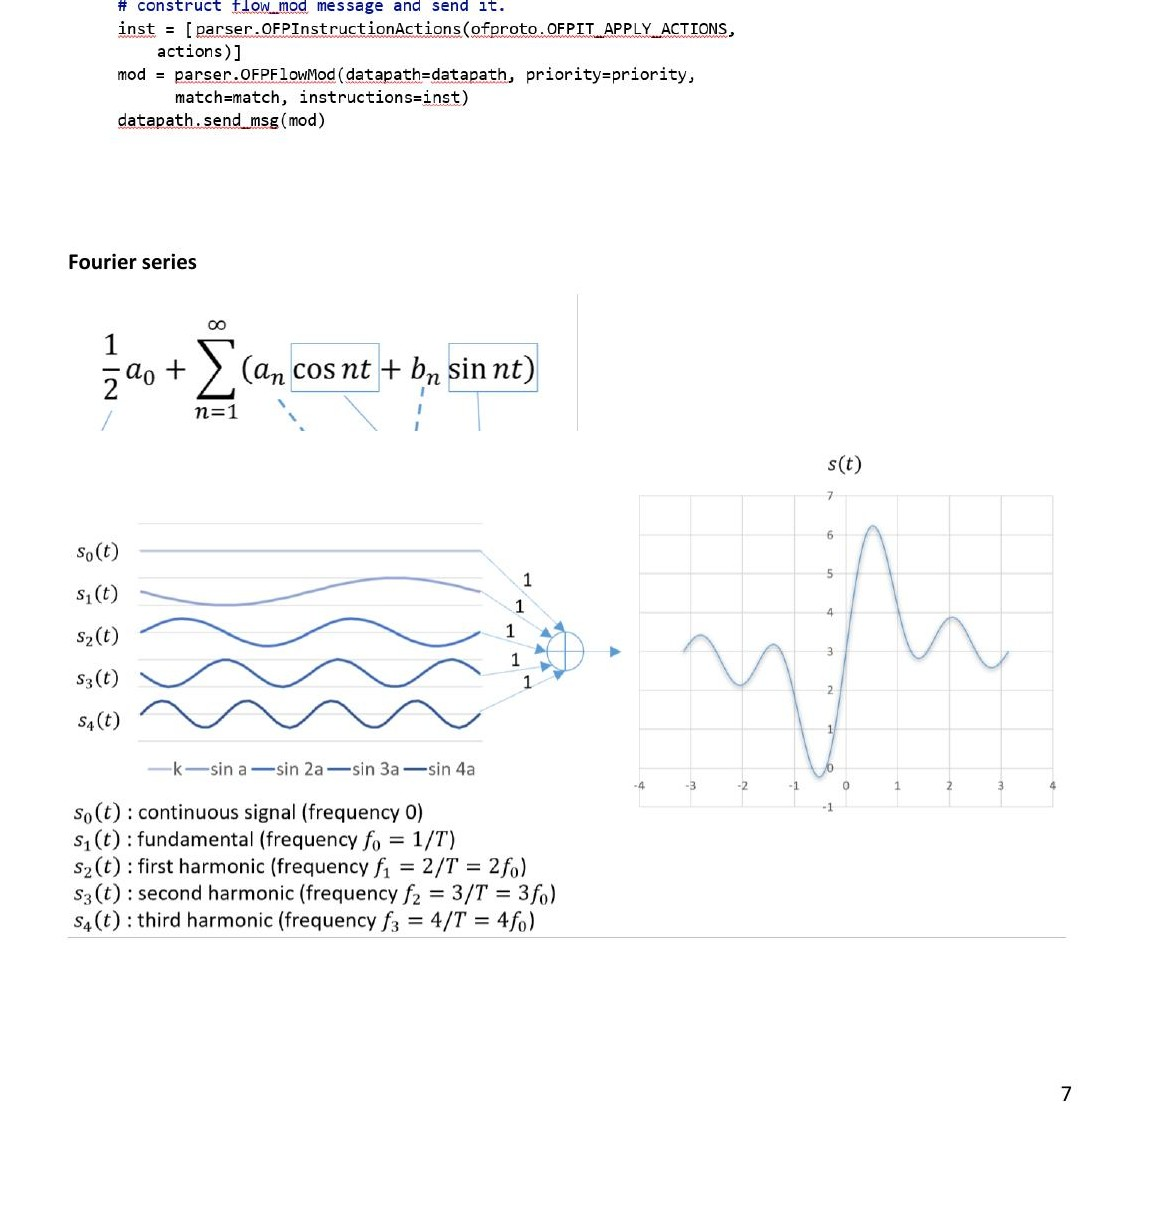
\includegraphics[keepaspectratio]{images/exam-mod2-fourier-series.jpg}}

Questo schema illustra il concetto fondamentale della \textbf{Serie di
Fourier}: qualsiasi segnale periodico può essere decomposto in una somma
(infinita) di funzioni sinusoidali a frequenze multiple della frequenza
fondamentale.

\subsection{L'Intuizione Fondamentale}\label{lintuizione-fondamentale}

Un segnale periodico può essere visto come una sovrapposizione di
componenti sinusoidali, ciascuna con frequenza, ampiezza e fase
specifiche. Questo cambio di prospettiva --- dal dominio del tempo al
\textbf{dominio della frequenza} --- è cruciale perché il canale
trasmissivo agisce in modo diverso su componenti a frequenza diversa.
Sapere quali frequenze compongono un segnale --- cioè conoscere il suo
\textbf{spettro} --- permette di: - Predire come il segnale si deformerà
attraverso il canale. - Dimensionare la \textbf{banda} necessaria
(quante armoniche servono per rappresentare il segnale fedelmente). -
Progettare filtri per rimuovere componenti indesiderate.

La serie di Fourier decompone una funzione come somma di infinite
funzioni oscillanti a frequenze diverse. È formalmente un cambio di
coordinate: dal dominio del tempo a quello della frequenza. La base di
questa decomposizione è un insieme di funzioni ortogonali.

\subsection{Segnali Periodici
Continui}\label{segnali-periodici-continui}

Un segnale continuo \(s(t): \mathbb{R} \to \mathbb{R}\) è
\textbf{periodico con periodo \(T\)} se
\[s(t) = s(t + T) \quad \forall t \in \mathbb{R}\] I segnali periodici
si possono studiare interamente nell'intervallo \([0, T]\). La frequenza
fondamentale è \(f = 1/T\).

\subsection{Definizione della Serie di
Fourier}\label{definizione-della-serie-di-fourier}

Data una funzione continua \(s(t): \mathbb{R} \to \mathbb{R}\) periodica
in \([-\pi, \pi]\):
\[s(t) = \frac{1}{2} a_0 + \sum_{n=1}^{\infty} \left( a_n \cos(nt) + b_n \sin(nt) \right)\]
con coefficienti:
\[a_0 = \frac{1}{\pi} \int_{-\pi}^{\pi} s(t)\, dt \qquad a_n = \frac{1}{\pi} \int_{-\pi}^{\pi} s(t) \cos(nt)\, dt \qquad b_n = \frac{1}{\pi} \int_{-\pi}^{\pi} s(t) \sin(nt)\, dt\]

\textbf{Interpretazione fisica:} Ogni segnale periodico è la ``somma di
sinusoidi''. Il termine \(\frac{1}{2} a_0\) è la \textbf{componente
continua} (il valor medio del segnale). I termini successivi sono le
\textbf{armoniche}: la \textbf{fondamentale} con frequenza
\(f_0 = 1/T\), la \textbf{prima armonica} con frequenza
\(f_1 = 2/T = 2f_0\), la seconda armonica a \(3f_0\), e così via.

\subsection{Condizioni di Dirichlet}\label{condizioni-di-dirichlet}

La serie di Fourier non è definita per qualsiasi funzione. Le
\textbf{condizioni di Dirichlet} garantiscono l'esistenza della serie: è
sufficiente che il segnale sia \emph{piecewise continuous} (composta da
un numero finito di pezzi continui su ogni sottointervallo finito, con
limite finito nei punti di discontinuità). In corrispondenza delle
discontinuità la serie converge alla media dei limiti sinistro e destro.

\subsection{Fenomeno di Gibbs}\label{fenomeno-di-gibbs}

Quando la serie di Fourier approssima una funzione con discontinuità
(come un'onda quadra), si osserva un \textbf{overshoot} intorno ai punti
di salto che non scompare mai, per quanto si aumenti il numero di
armoniche. Questo è il \textbf{fenomeno di Gibbs}: l'errore rimane del
\textasciitilde9\% dell'ampiezza del salto, indipendentemente
dall'ordine di troncamento. Le oscillazioni nel tratto piatto si
riducono, ma il picco al salto rimane costante.

\newpage

\chapter{Network Slicing con SDN}\label{network-slicing-con-sdn}

\pandocbounded{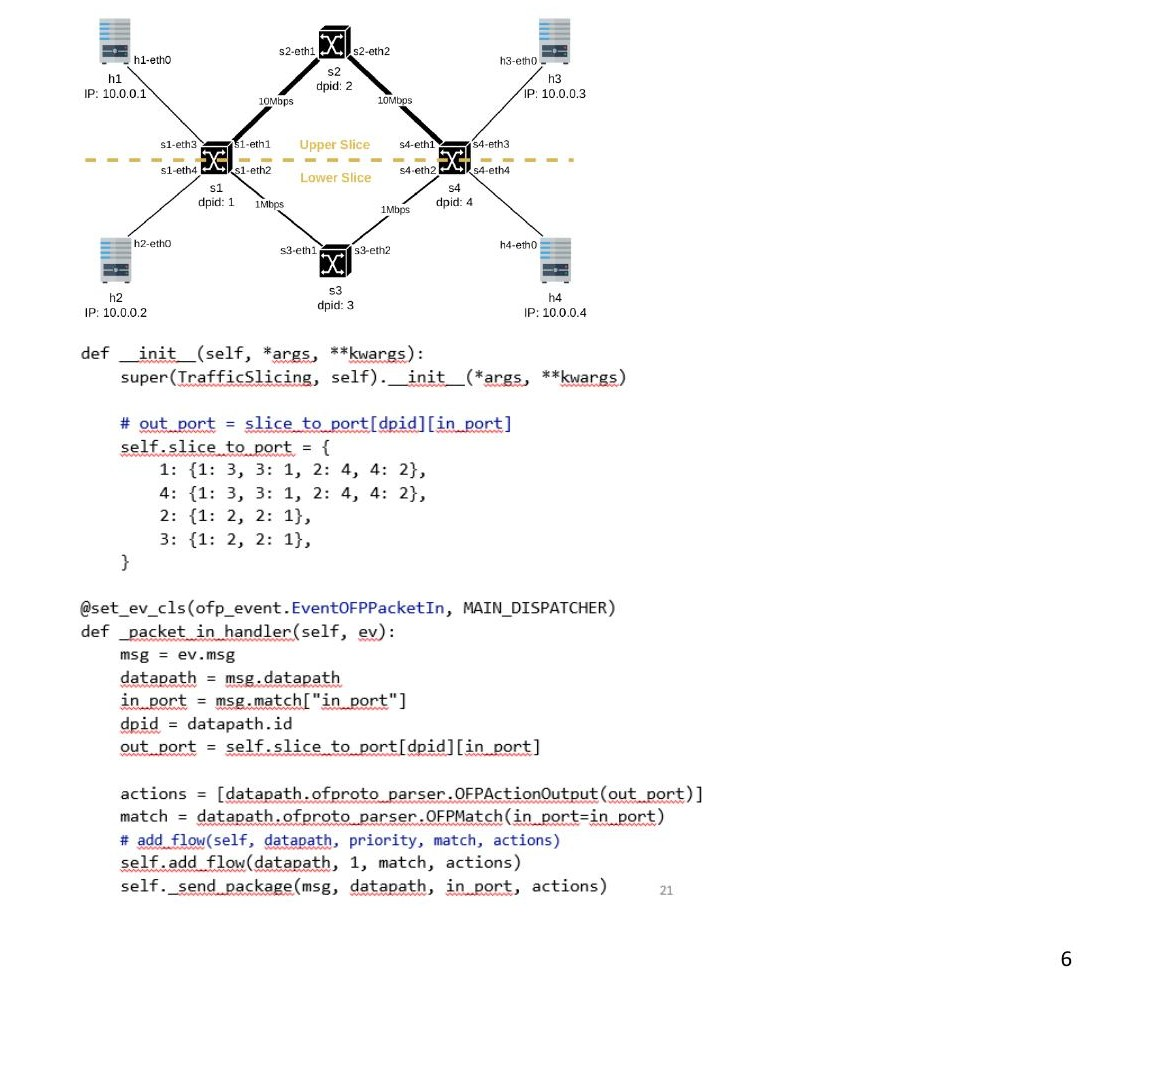
\includegraphics[keepaspectratio]{images/exam-mod2-network-slicing.jpg}}

\section{Contesto: il 5G e la necessità del Network
Slicing}\label{contesto-il-5g-e-la-necessituxe0-del-network-slicing}

Il 5G non è semplicemente un incremento di velocità rispetto al 4G: è
una riprogettazione fondamentale dell'architettura di rete, motivata
dalla coesistenza di tre categorie di servizio con requisiti
radicalmente diversi tra loro: - \textbf{mMTC (massive Machine Type
Communications)}: comunicazione tra un numero elevatissimo di
dispositivi (fino a 200.000/km²), IoT a bassa potenza. I requisiti
dominanti sono la massima efficienza energetica e la scalabilità. -
\textbf{URLLC (Ultra-Reliable Low-Latency Communications)}: servizi che
richiedono simultaneamente bassissima latenza (≤ 5 ms o ≤ 1 ms) e alta
affidabilità (es. guida autonoma, controllo industriale). - \textbf{eMBB
(Enhanced Mobile Broadband)}: servizi ad alta densità di dati (streaming
4K/8K, realtà aumentata), dove il requisito primario è l'alta capacità
di trasmissione.

La coesistenza di questi tre profili rende impossibile ottimizzare
un'unica rete per tutti contemporaneamente. La soluzione è il
\textbf{network slicing}: sulla stessa infrastruttura fisica vengono
create più reti virtuali logiche separate (\emph{slice}), ognuna
ottimizzata per il proprio caso d'uso, con le proprie caratteristiche di
QoS, banda, latenza e isolamento. La separazione logica garantisce che i
requisiti di una slice non vengano degradati dalle altre.

\section{Il concetto di Network
Slicing}\label{il-concetto-di-network-slicing}

Il network slicing sfrutta le risorse dell'infrastruttura fisica per
creare multiple \textbf{sotto-reti virtuali} (slice), ciascuna delle
quali si comporta come una rete indipendente.

Senza SDN, separare il traffico richiederebbe VLAN, configurazione
manuale di ogni switch, o hardware dedicato. Con \textbf{SDN}
(Software-Defined Networking), è sufficiente un controller centralizzato
che installa le regole di forwarding appropriate per ogni flusso,
realizzando lo slicing in software.

\section{Topologia dell'esperimento}\label{topologia-dellesperimento}

L'esperimento implementa il network slicing usando l'emulatore
\textbf{ComNetsEmu} e il controller SDN \textbf{Ryu} (scritto in
Python).

La topologia è un \textbf{anello di quattro switch} (S1, S2, S3, S4) con
quattro host (h1, h2, h3, h4). L'obiettivo è imporre un
\textbf{partizionamento rigido} della topologia per creare due slice
indipendenti: - \textbf{Upper Slice}: h1 ↔ h3, interconnessi
esclusivamente tramite i link a 10 Mbps (il percorso via S2). -
\textbf{Lower Slice}: h2 ↔ h4, interconnessi esclusivamente tramite i
link a 1 Mbps (il percorso via S3).

\section{Implementazione con Ryu:
TrafficSlicing}\label{implementazione-con-ryu-trafficslicing}

Il cuore dell'implementazione del Network Slicing nel codice Python per
il controller Ryu è il dizionario \texttt{slice\_to\_port}. Per ogni
switch (identificato dal \texttt{dpid}) e per ogni porta di ingresso
(\texttt{in\_port}), specifica la porta di uscita:

\begin{Shaded}
\begin{Highlighting}[]
\VariableTok{self}\NormalTok{.slice\_to\_port }\OperatorTok{=}\NormalTok{ \{}
    \DecValTok{1}\NormalTok{: \{}\DecValTok{1}\NormalTok{: }\DecValTok{3}\NormalTok{, }\DecValTok{3}\NormalTok{: }\DecValTok{1}\NormalTok{, }\DecValTok{2}\NormalTok{: }\DecValTok{4}\NormalTok{, }\DecValTok{4}\NormalTok{: }\DecValTok{2}\NormalTok{\},  }\CommentTok{\# S1 (dpid=1)}
    \DecValTok{4}\NormalTok{: \{}\DecValTok{1}\NormalTok{: }\DecValTok{3}\NormalTok{, }\DecValTok{3}\NormalTok{: }\DecValTok{1}\NormalTok{, }\DecValTok{2}\NormalTok{: }\DecValTok{4}\NormalTok{, }\DecValTok{4}\NormalTok{: }\DecValTok{2}\NormalTok{\},  }\CommentTok{\# S4 (dpid=4)}
    \DecValTok{2}\NormalTok{: \{}\DecValTok{1}\NormalTok{: }\DecValTok{2}\NormalTok{, }\DecValTok{2}\NormalTok{: }\DecValTok{1}\NormalTok{\},               }\CommentTok{\# S2 (dpid=2)}
    \DecValTok{3}\NormalTok{: \{}\DecValTok{1}\NormalTok{: }\DecValTok{2}\NormalTok{, }\DecValTok{2}\NormalTok{: }\DecValTok{1}\NormalTok{\},               }\CommentTok{\# S3 (dpid=3)}
\NormalTok{\}}
\end{Highlighting}
\end{Shaded}

Il gestore \texttt{\_packet\_in\_handler} viene chiamato dal controller
Ryu ogni volta che uno switch riceve un pacchetto che non ha una flow
entry corrispondente (\emph{packet-in}). Il controller legge il
\texttt{dpid} dello switch e la porta di ingresso, cerca nel dizionario
la porta di uscita, installa una \textbf{flow rule} nello switch (con
\texttt{self.add\_flow}) e forwarda il pacchetto:

\begin{Shaded}
\begin{Highlighting}[]
\KeywordTok{def}\NormalTok{ \_packet\_in\_handler(}\VariableTok{self}\NormalTok{, ev):}
\NormalTok{    msg }\OperatorTok{=}\NormalTok{ ev.msg}
\NormalTok{    datapath }\OperatorTok{=}\NormalTok{ msg.datapath}
\NormalTok{    in\_port }\OperatorTok{=}\NormalTok{ msg.match[}\StringTok{"in\_port"}\NormalTok{]}
\NormalTok{    dpid }\OperatorTok{=}\NormalTok{ datapath.}\BuiltInTok{id}

\NormalTok{    out\_port }\OperatorTok{=} \VariableTok{self}\NormalTok{.slice\_to\_port[dpid][in\_port]}

\NormalTok{    actions }\OperatorTok{=}\NormalTok{ [datapath.ofproto\_parser.OFPActionOutput(out\_port)]}
\NormalTok{    match }\OperatorTok{=}\NormalTok{ datapath.ofproto\_parser.OFPMatch(in\_port}\OperatorTok{=}\NormalTok{in\_port)}
    \VariableTok{self}\NormalTok{.add\_flow(datapath, }\DecValTok{1}\NormalTok{, match, actions)}
    \VariableTok{self}\NormalTok{.\_send\_package(msg, datapath, in\_port, actions)}
\end{Highlighting}
\end{Shaded}

Da quel momento in poi, i pacchetti che corrispondono al match vengono
gestiti direttamente dallo switch senza coinvolgere il controller.
L'isolamento è garantito logicamente dal partizionamento delle porte su
S1 e S4.

\newpage

\chapter{Campionamento, Quantizzazione e
DFT}\label{campionamento-quantizzazione-e-dft}

\section{Da Segnale Analogico a Digitale: Campionamento e
Quantizzazione}\label{da-segnale-analogico-a-digitale-campionamento-e-quantizzazione}

I sistemi digitali moderni lavorano esclusivamente con dati discreti. Un
segnale analogico continuo deve essere convertito in una sequenza di
valori discreti. Questo processo si articola in due fasi:
\textbf{campionamento} e \textbf{quantizzazione}. Dopo il filtraggio
anti-aliasing (passa-basso con \(f_{taglio} = f_c/2\)), avviene il
campionamento, seguito dalla quantizzazione e infine dalla codifica
binaria.

\subsection{Il Campionamento e il Teorema di
Nyquist-Shannon}\label{il-campionamento-e-il-teorema-di-nyquist-shannon}

\textbf{Campionare} un segnale \(s(t)\) significa estrarre i valori che
il segnale assume a istanti discreti regolarmente spaziati. Il parametro
chiave è la frequenza di campionamento \(f_c = 1/T_c\).

Affinché un segnale di banda \(B\) (frequenza massima \(f_{max}\)) sia
ricostruito perfettamente dai suoi campioni, la frequenza di
campionamento deve soddisfare il \textbf{Teorema di Nyquist-Shannon}:
\[f_c \geq 2 \cdot f_{max}\]

La frequenza \(f_{Nyquist} = f_c/2\) è la massima frequenza
rappresentabile senza aliasing.

\subsection{Aliasing}\label{aliasing}

\pandocbounded{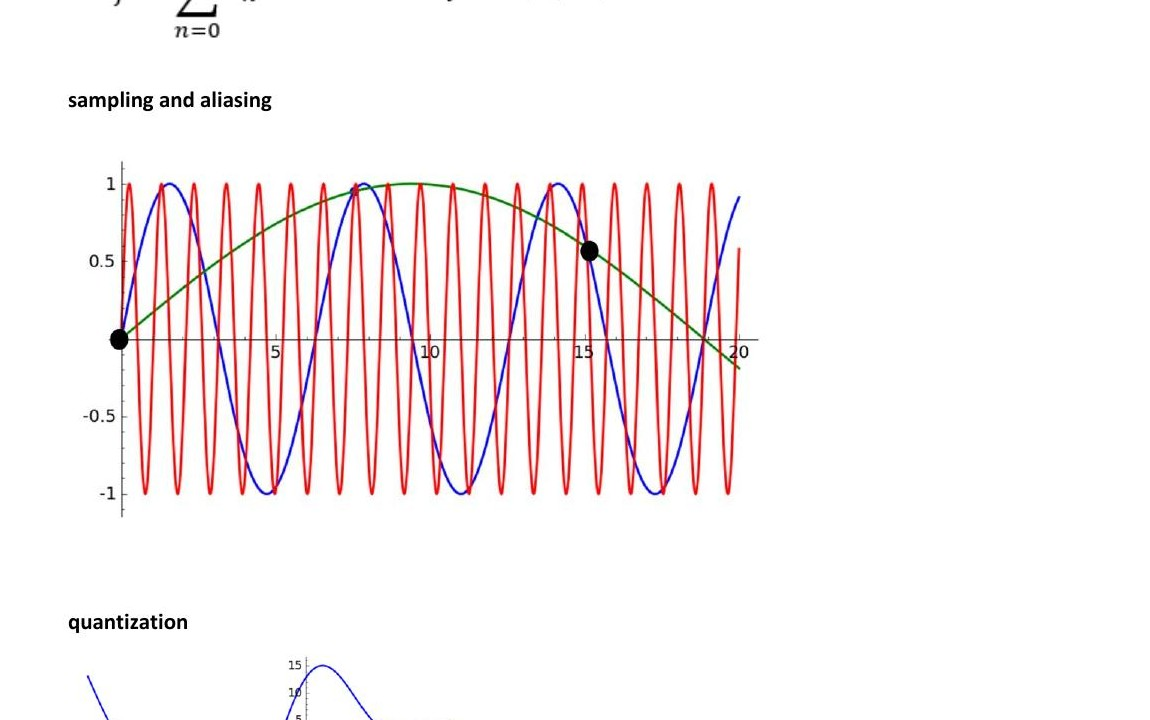
\includegraphics[keepaspectratio]{images/exam-mod2-sampling-aliasing.jpg}}

Campionare introduce un'ambiguità: da un insieme finito di campioni non
si può distinguere univocamente quale segnale li ha generati.
L'\textbf{aliasing} è la distorsione che si verifica quando il segnale
rosso (alta frequenza) e il segnale blu (bassa frequenza) producono
\textbf{identici campioni} (i punti neri). Il segnale a bassa frequenza
è l'\textbf{alias} di quello ad alta frequenza: un'identità fantasma
creata dal sottocampionamento.

Se nel segnale originale sono presenti frequenze superiori a
\(f_{Nyquist}\), queste appaiono come frequenze più basse nello spettro
discreto, rendendo impossibile la ricostruzione.

\textbf{Come prevenire l'aliasing:} si applica un \textbf{filtro
anti-aliasing} (filtro passa-basso analogico) prima del campionatore,
che elimina tutte le componenti con \(f > f_c/2\). Solo dopo si
campiona. Questo garantisce che il segnale digitale rappresenti
fedelmente l'originale entro la banda di interesse. Esempi: - Audio CD:
frequenza di campionamento 44.1 kHz, per limiti uditivi di
\textasciitilde20 kHz. - Telefonia: 8 kHz. - WiFi e reti cellulari: i
ricevitori campionano il segnale RF ad almeno \(2 \times B_{canale}\).

\subsection{Quantizzazione}\label{quantizzazione}

\pandocbounded{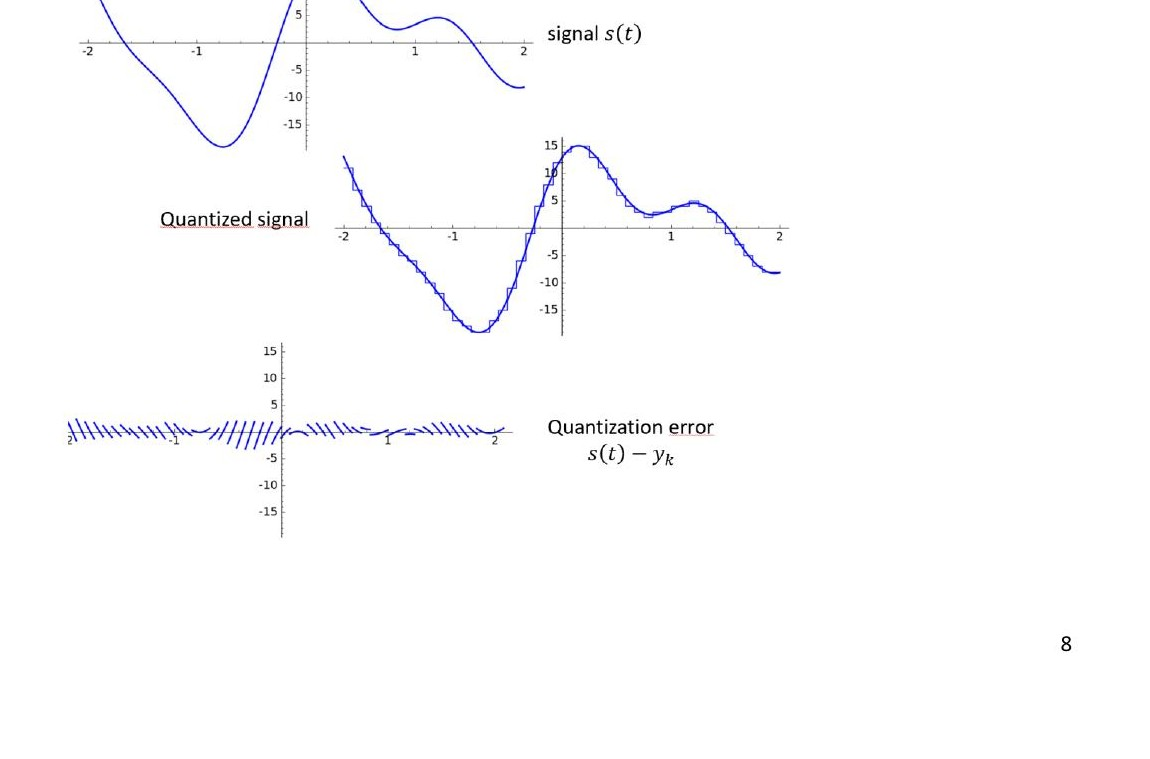
\includegraphics[keepaspectratio]{images/exam-mod2-quantization.jpg}}

La \textbf{quantizzazione} è il secondo passo nella conversione
analogico-digitale. Dopo aver campionato il segnale nel tempo, ogni
campione deve essere approssimato al livello discreto più vicino tra un
insieme finito di valori possibili (usando un numero finito di bit).

Dato un campione con valore reale, si sceglie il \textbf{livello di
quantizzazione} \(y_k\) più vicino e si assegna il codice binario. Se si
usano \(M\) bit per campione, si hanno \(2^M\) livelli di
quantizzazione, spaziati di un passo
\(\Delta = \frac{s_{max} - s_{min}}{2^M}\).

\textbf{L'errore di quantizzazione:} l'approssimazione introduce un
errore inevitabile \(e = s(t) - y_k\), che ha valore assoluto al massimo
\(\Delta/2\). Nel grafico in basso si vede chiaramente che l'errore è un
segnale oscillante (dovuto all'arrotondamento al gradino) con ampiezza
piccola (\(\approx \Delta/2\)) e frequenza elevata. Questo errore viene
tipicamente modellato come rumore bianco uniforme.

\textbf{Trade-off:} - Aumentare \(M\) (più bit per campione) riduce
\(\Delta\) e quindi l'errore di quantizzazione, ma aumenta il
\textbf{bitrate} richiesto: \(\text{Bitrate} = f_c \times M\) bit/s. -
Il \textbf{SNR di quantizzazione} cresce approssimativamente di 6 dB per
ogni bit aggiunto: \(\text{SNR}_{dB} \approx 6.02 \cdot M + 1.76\) dB.

\section{Trasformata Discreta di Fourier
(DFT)}\label{trasformata-discreta-di-fourier-dft}

La \textbf{Trasformata di Fourier Discreta} (DFT) è la versione
\emph{calcolabile da un computer} dell'analisi di Fourier: opera su un
segnale discreto di lunghezza finita \(N\) e produce \(N\) coefficienti
frequenziali.

\textbf{La formula:} dato un segnale campionato \(s_n\) (con
\(n = 0, 1, \ldots, N-1\)), la DFT calcola il coefficiente \(S_f\) per
ogni frequenza discreta \(f = 0, 1, \ldots, N-1\):
\[S_f = \sum_{n=0}^{N-1} s_n \, e^{-j\frac{2\pi f}{N}n}\]

\textbf{Interpretazione:} - Ogni coefficiente \(S_f\) è un numero
complesso: il suo \textbf{modulo} \(|S_f|\) è l'ampiezza del contributo
alla frequenza \(f\), la sua \textbf{fase} \(\arg(S_f)\) è lo sfasamento
della componente sinusoidale corrispondente. - La DFT assume
implicitamente che il segnale di \(N\) campioni sia la ripetizione
periodica di un pattern. È il corrispettivo discreto della serie di
Fourier.

\textbf{L'algoritmo FFT:} Il calcolo diretto della DFT ha complessità
\(O(N^2)\). L'algoritmo \textbf{FFT} (\emph{Fast Fourier Transform})
riduce la complessità a \(O(N \log N)\) sfruttando la simmetria del
fattore. Per \(N = 1024\) punti, la FFT è ≈100 volte più veloce della
DFT diretta. \textbf{Applicazioni pratiche:} Analisi spettrale,
filtraggio digitale (e compressione JPEG tramite DCT), e implementazione
dell'\textbf{OFDM} (Orthogonal Frequency Division Multiplexing) in
4G/5G, che crea il segnale con una IFFT e lo demodula con una FFT.

\newpage

\chapter{Lezione 5 - (Lab) Wireless}\label{lezione-5---lab-wireless}

\section{Il Problema del Terminale Nascosto (Hidden Terminal
Problem)}\label{il-problema-del-terminale-nascosto-hidden-terminal-problem}

A causa dell'attenuazione con la distanza (o per la presenza di ostacoli
fisici come montagne e palazzi), due nodi potrebbero non essere in grado
di percepirsi a vicenda, pur essendo entrambi nel raggio di un terzo
nodo intermedio. Se A e C vogliono comunicare con B, ma A e C sono fuori
portata l'uno per l'altro, entrambi potrebbero iniziare a trasmettere
contemporaneamente --- inconsapevoli della reciproca interferenza ---
causando una collisione disastrosa al ricevitore B. Questo è il
\textbf{Problema del Terminale Nascosto} (\emph{Hidden Terminal
Problem}), e non può essere rilevato dal classico meccanismo CSMA/CD.

\pandocbounded{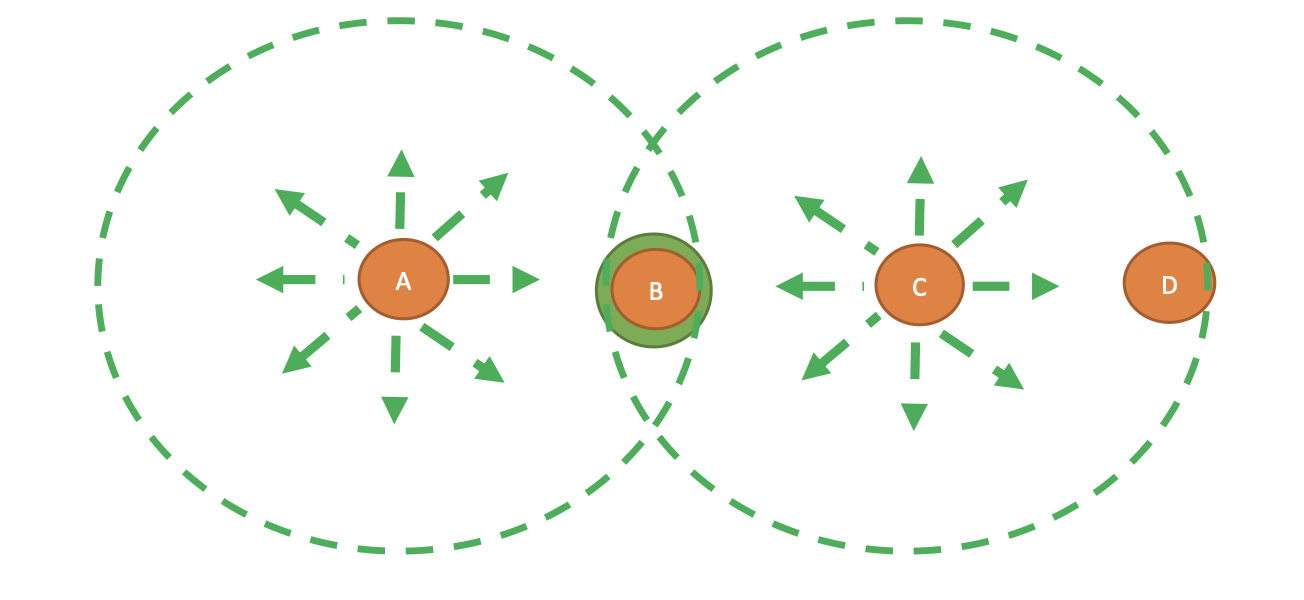
\includegraphics[keepaspectratio]{images/Pasted-image-20260429160400.png}}

Il problema del \textbf{terminale nascosto} nasce da una limitazione
fisica fondamentale delle reti wireless: la potenza del segnale radio
cala con il quadrato della distanza, e la comunicazione può avvenire
solo tra nodi sufficientemente vicini. In questo scenario, A e C
vogliono entrambi trasmettere a B, ma A e C si trovano fuori dal raggio
radio l'uno dell'altro.

Supponiamo che A stia già trasmettendo verso B. La stazione C, prima di
trasmettere, esegue il \textbf{Carrier Sense}: ascolta il canale per
verificare se è libero. Poiché C non riesce a sentire il segnale di A
(sono fuori portata), C conclude erroneamente che il canale sia libero e
inizia a trasmettere verso B (o verso D). Il risultato è che i segnali
di A e di C si sovrappongono fisicamente nell'antenna di B, generando
una \textbf{collisione} che B riceve come segnale incomprensibile. Né A
né C rilevano la collisione, perché ciascuna sente solo il proprio
segnale (che è enormemente più forte di qualsiasi segnale di ritorno).

Questo è il motivo per cui il protocollo \textbf{CSMA/CD}, standard
nelle reti Ethernet cablate, non può essere usato nelle reti wireless:
il meccanismo di rilevamento delle collisioni richiede che il
trasmettitore possa ascoltare il canale mentre trasmette, il che è
impossibile in radio (il self-signal del trasmettitore è ordini di
grandezza più forte di qualsiasi segnale debole in arrivo).

\begin{callouttip}{Il punto chiave}

Con CSMA classico, il Carrier Sense viene eseguito dal trasmettitore, ma
quello che conta è lo stato del canale \textbf{al ricevitore}. Il
terminale nascosto è ``nascosto'' solo rispetto al trasmettitore
corrente, non rispetto al ricevitore.

\end{callouttip}

La soluzione a questo problema è il meccanismo \textbf{RTS/CTS}.

\newpage

\chapter{Lezione 6 - (Lab) Protocolli MAC e Reti
Wireless}\label{lezione-6---lab-protocolli-mac-e-reti-wireless}

\section{Le Reti Wireless: Sfide e Problemi
Strutturali}\label{le-reti-wireless-sfide-e-problemi-strutturali}

Nelle reti cablate il rilevamento delle collisioni in fase di
trasmissione funziona perfettamente, ma nelle reti wireless questo
principio fallisce a causa della natura stessa del mezzo radio. Nelle
trasmissioni senza fili, la potenza del segnale decade rapidamente,
diminuendo in proporzione al quadrato della distanza.

A causa di questa attenuazione, il segnale emesso dall'antenna del
trasmettitore (il \emph{self-signal}) risulta infinitamente più forte
rispetto a qualsiasi altro segnale debole in arrivo da una stazione
distante. Questo ``acceca'' il trasmettitore, rendendogli impossibile
rilevare una collisione mentre sta inviando dati. Inoltre, le condizioni
del canale wireless sono spazialmente diverse tra chi trasmette e chi
riceve. Una collisione rilevata dal trasmettitore potrebbe non essere
una collisione al ricevitore, e viceversa. Nelle reti wireless, l'unica
cosa che conta veramente è l'\textbf{interferenza al ricevitore}, non al
mittente. Questa limitazione genera due problemi classici della
comunicazione radio: il \emph{Terminale Nascosto} e il \emph{Terminale
Esposto}.

\subsection{Il Problema del Terminale Nascosto (Hidden
Terminal)}\label{il-problema-del-terminale-nascosto-hidden-terminal}

\pandocbounded{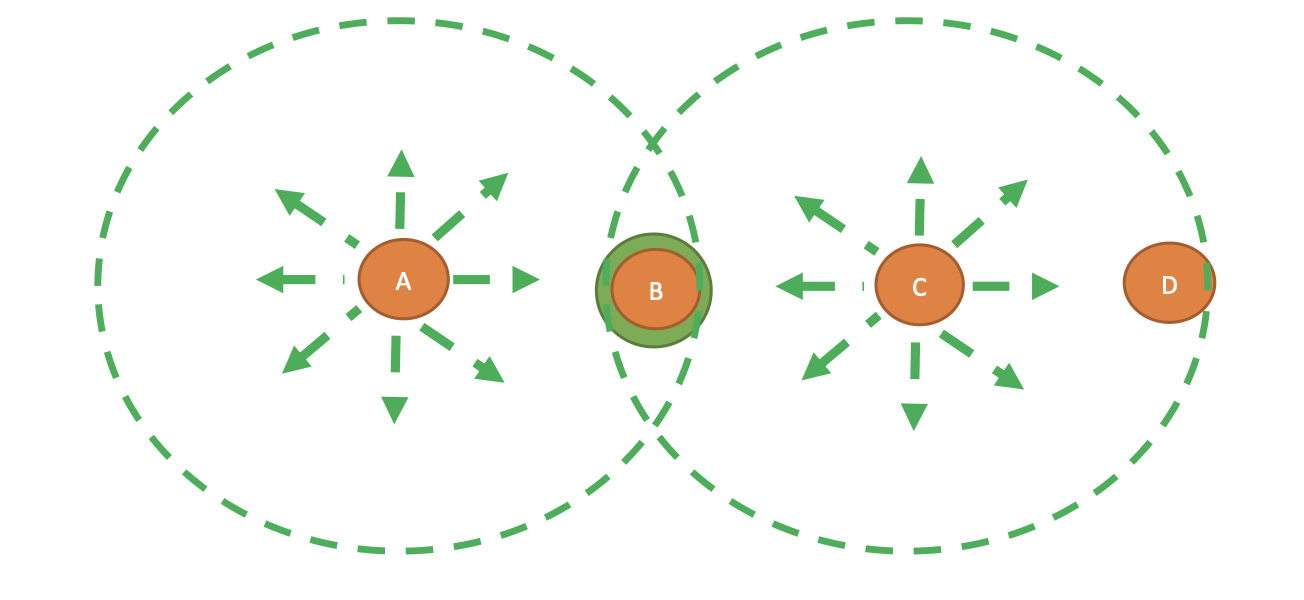
\includegraphics[keepaspectratio]{images/Pasted-image-20260429160400.png}}

\begin{calloutdefinition}{Terminale Nascosto (Hidden Terminal)}

Si verifica quando due o più stazioni, reciprocamente fuori dal raggio
radio l'una dell'altra, trasmettono simultaneamente verso un
destinatario comune. Poiché nessuna delle due stazioni riesce a rilevare
la trasmissione dell'altra, entrambe credono il canale libero e avviano
l'invio, causando una collisione al ricevitore che nessuna delle
sorgenti è in grado di percepire.

\end{calloutdefinition}

Immaginiamo quattro stazioni allineate: A, B, C e D. A è in raggio radio
con B; B è nel raggio di A e C; C è nel raggio di B e D. Supponiamo che
A stia attualmente trasmettendo dei dati a B. C, desiderando
trasmettere, si mette in ascolto sul mezzo. Poiché C si trova
fisicamente al di fuori del raggio di copertura radio di A, non
percepirà alcuna trasmissione in corso. Credendo che il canale sia
libero, C avvia una trasmissione (diretta a B o a D). Il risultato è
disastroso: i segnali di A e di C si sovrapporranno fisicamente in
corrispondenza dell'antenna di B, causando una collisione e distruggendo
i dati. In questo scenario, C è incapace di rilevare il potenziale
competitore (A) ed è quindi definito come \textbf{nascosto} (hidden)
rispetto alla comunicazione da A verso B. Il problema del terminale
nascosto si verifica quando due o più stazioni, reciprocamente fuori
raggio, trasmettono simultaneamente a un destinatario comune. Anche A,
per lo stesso motivo legato alla distanza, non si accorgerà della
collisione provocata da C.

Questo è il motivo per cui il protocollo \textbf{CSMA/CD}, standard
nelle reti Ethernet cablate, non può essere usato nelle reti wireless:
il meccanismo di rilevamento delle collisioni richiede che il
trasmettitore possa ascoltare il canale mentre trasmette, il che è
impossibile in radio (il self-signal del trasmettitore è ordini di
grandezza più forte di qualsiasi segnale debole in arrivo).

\begin{callouttip}{Il punto chiave}

Con CSMA classico, il Carrier Sense viene eseguito dal trasmettitore, ma
quello che conta è lo stato del canale \textbf{al ricevitore}. Il
terminale nascosto è ``nascosto'' solo rispetto al trasmettitore
corrente, non rispetto al ricevitore.

\end{callouttip}

La soluzione a questo problema è il meccanismo \textbf{RTS/CTS}.

\subsection{Il Problema del Terminale Esposto (Exposed
Terminal)}\label{il-problema-del-terminale-esposto-exposed-terminal}

\pandocbounded{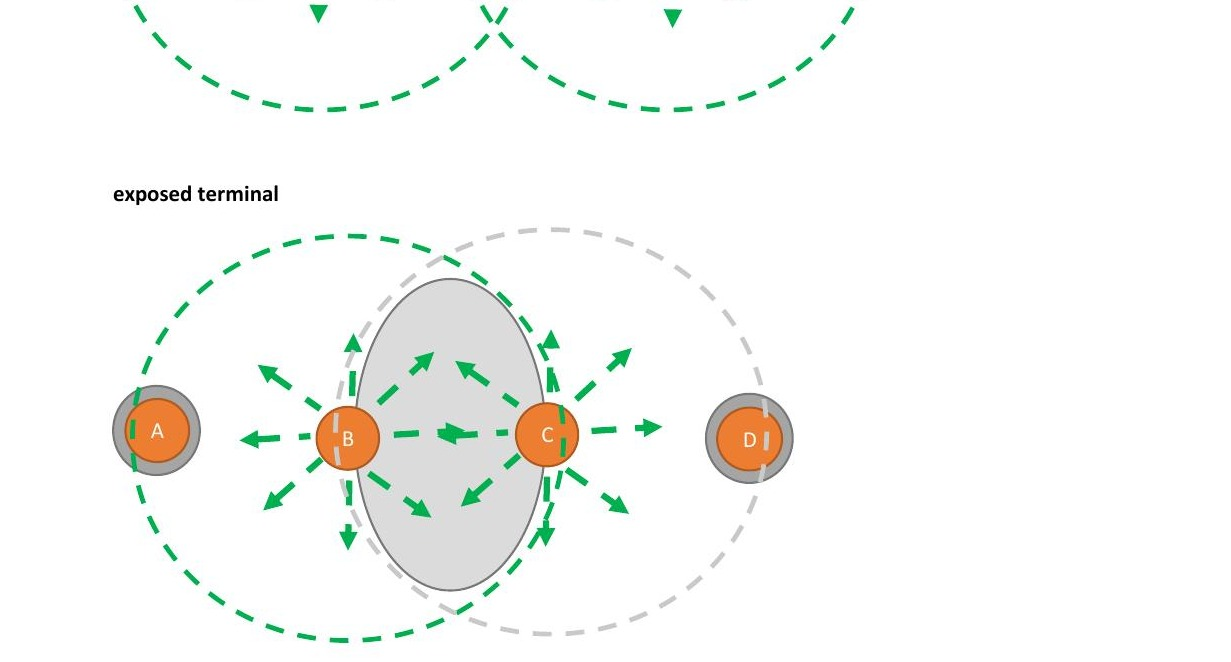
\includegraphics[keepaspectratio]{images/exam-mod2-exposed-terminal.jpg}}

\begin{calloutdefinition}{Terminale Esposto (Exposed Terminal)}

Si verifica quando una stazione rinuncia inutilmente a trasmettere
perché rileva sul canale il segnale di un'altra stazione, pur non
essendoci alcun rischio di collisione al ricevitore di destinazione. La
stazione ``esposta'' è in grado di ascoltare una trasmissione vicina ma
irrilevante, e ne viene erroneamente bloccata dall'invio di frame del
tutto legittimi verso un destinatario distante.

\end{calloutdefinition}

Il problema del \textbf{terminale esposto} è speculare al precedente:
questa volta, una stazione si astiene inutilmente dal trasmettere perché
percepisce un segnale sul canale, anche se quel segnale non crea
interferenza al suo ricevitore di destinazione.

Consideriamo la stessa topologia (A, B, C, D). Questa volta, B sta
trasmettendo dati verso A, e parallelamente C desidera inviare un
messaggio a D. C, mettendosi in ascolto, rileva forte e chiaro il
segnale di B. Applicando ciecamente le regole del CSMA, C conclude
erroneamente di non poter trasmettere verso D, per paura di creare una
collisione. In realtà, se C iniziasse a trasmettere, il suo segnale
raggiungerebbe D senza problemi, e le due trasmissioni (da B verso A, e
da C verso D) potrebbero avvenire perfettamente in parallelo senza
disturbarsi a vicenda (le loro ``zone di interferenza'' ai ricevitori
non si sovrappongono in modo distruttivo). In questo caso, C è un
terminale \textbf{esposto} alla comunicazione tra B e A. Il problema del
terminale esposto impedisce a una stazione trasmittente di inviare frame
del tutto legittimi a causa dell'ascolto di un'interferenza locale
generata da un'altra stazione.

\begin{calloutwarning}{Attenzione}

Il terminale esposto non è un problema di collisione, ma di
\textbf{sotto-utilizzo del canale}. È meno grave del terminale nascosto
(che causa corruzioni di dati), ma riduce il throughput complessivo
della rete.

\end{calloutwarning}

Il fatto che non si possa verificare lo stato del canale al ricevitore
semplicemente mettendosi in ascolto dal trasmettitore rende palese la
necessità di progettare protocolli MAC sensibilmente diversi da quelli
delle classiche reti LAN cablate. Il meccanismo RTS/CTS del protocollo
MACA risolve anche questo problema.

\section{I Protocolli MACA e MACAW: Evitare le
Collisioni}\label{i-protocolli-maca-e-macaw-evitare-le-collisioni}

Per mitigare le problematiche descritte, nel 1990 Phil Karn presentò un
protocollo rivoluzionario chiamato \textbf{MACA} (Multiple Access with
Collision Avoidance), originariamente concepito per il ``packet radio''.
L'idea fondante del MACA non è quella di rilevare le collisioni, ma di
prevenirle stimolando il ricevitore a inviare un breve frame di
controllo prima che inizi la trasmissione dei dati veri e propri (molto
più lunghi). Le stazioni vicine, sentendo questo frame di controllo, si
asterranno dal trasmettere durante il successivo invio dei dati.

\subsection{Il Meccanismo RTS / CTS}\label{il-meccanismo-rts-cts}

\pandocbounded{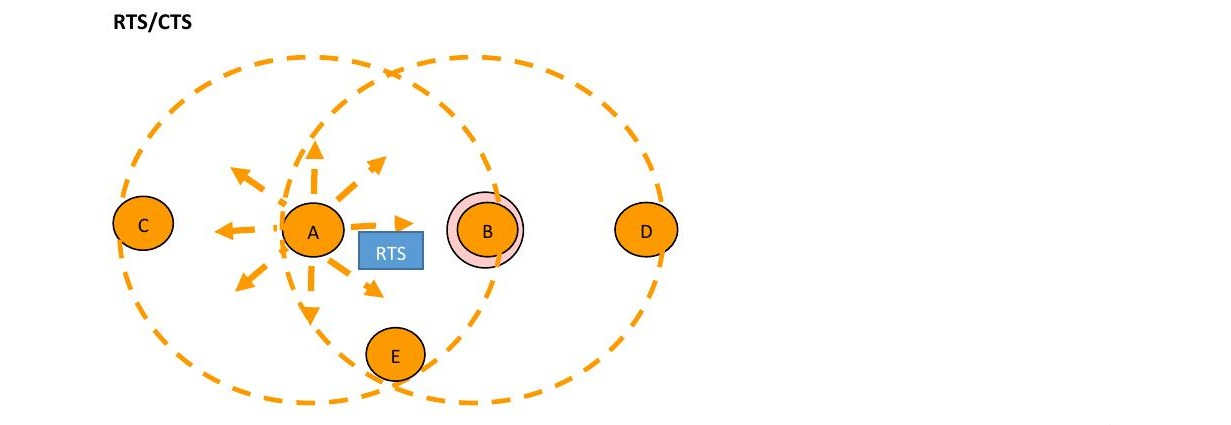
\includegraphics[keepaspectratio]{images/exam-mod2-rts-cts.jpg}}

Il meccanismo \textbf{RTS/CTS} (\emph{Request To Send / Clear To Send})
è il cuore del protocollo \textbf{MACA} e del successivo \textbf{MACAW},
ed è integrato nello standard \textbf{IEEE 802.11} (Wi-Fi). Risolve
entrambi i problemi del terminale nascosto e del terminale esposto
prenotando il canale in modo distribuito prima di trasmettere i dati.

Il funzionamento si basa su uno scambio di messaggi denominato RTS/CTS e
si articola in tre fasi:

\begin{enumerate}
\def\labelenumi{\arabic{enumi}.}
\item
  \textbf{Fase 1 --- RTS (Request To Send):} Quando la stazione A
  desidera inviare dati a B, invia prima un breve pacchetto RTS (≈20
  byte) indirizzato a B. Questo pacchetto non è generico, ma contiene
  l'ID della sorgente (A), l'ID della destinazione (B) e, fattore
  cruciale, la lunghezza (durata) del frame dati che seguirà. Tutte le
  stazioni nel raggio di A (ad esempio C ed E) riceveranno questo RTS.
\item
  \textbf{Fase 2 --- CTS (Clear To Send):} Se B riceve l'RTS ed è pronto
  e libero per ricevere il messaggio, risponde trasmettendo un pacchetto
  CTS. Anche il CTS è un frame molto breve che copia e diffonde
  l'informazione sulla durata dei dati dichiarata nell'RTS. Questo CTS
  verrà ascoltato da A (che ottiene così il permesso di procedere), ma
  anche da tutte le stazioni nel raggio di B (ad esempio D ed E).
\item
  \textbf{Fase 3 --- DATA:} Alla ricezione del frame CTS, la stazione A
  inizia a trasmettere il frame dati vero e proprio in condizioni
  sicure.
\end{enumerate}

\begin{callouttip}{Insight chiave del meccanismo RTS/CTS}

Il meccanismo RTS/CTS risolve entrambi i problemi topologici in modo
elegante: il terminale nascosto viene messo a tacere dal CTS del
ricevitore (che esso sente, anche se non ha sentito l'RTS del mittente),
mentre il terminale esposto viene liberato dall'obbligo di silenzio
perché sente l'RTS ma non il CTS (e quindi deduce che la ricezione
avviene fuori dalla sua area di influenza). Il canale viene così
``prenotato'' in modo distribuito, senza coordinamento centralizzato.

\end{callouttip}

Vediamo in dettaglio come il MACA risolve i problemi topologici
precedenti:

\begin{itemize}
\tightlist
\item
  \textbf{Come risolve il terminale esposto (C nel diagramma):} La
  stazione C ascolta l'RTS inviato da A, ma, essendo troppo lontana da
  B, non sentirà mai il relativo CTS di B. Da questo C deduce di essere
  un terminale esposto: comprende che la ricezione avviene lontano dalla
  sua area di influenza ed è quindi del tutto libera di iniziare una
  propria trasmissione senza creare interferenze.
\item
  \textbf{Come risolve il terminale nascosto (D nel diagramma):} La
  stazione D non ascolta l'RTS di A (troppo lontano), ma riceve forte e
  chiaro il CTS di risposta inviato da B. D capisce immediatamente che B
  è in procinto di ricevere dati e che una sua trasmissione
  disturberebbe B. Pertanto, D si silenzia disciplinatamente per la
  durata indicata nel CTS, evitando di interferire con la ricezione di
  B.
\item
  \textbf{Il caso E:} Se una stazione centrale come E si trova nella
  zona di sovrapposizione e ascolta sia l'RTS che il CTS, sa con
  certezza di dover rimanere in silenzio per tutta la durata della
  comunicazione per non disturbare l'operazione in corso.
\end{itemize}

\begin{callouttip}{Collisioni residue}

Con RTS/CTS le collisioni non scompaiono del tutto: possono ancora
avvenire tra pacchetti RTS (es. se C e D inviano contemporaneamente RTS
verso A). Ma in tal caso nessun dato applicativo viene perso (NO DATA
information is lost), e lo spreco di canale è minimo dato che gli RTS
sono brevissimi (circa 20 byte). I mittenti applicano il \textbf{Binary
Exponential Backoff} prima di riprovare.

\end{callouttip}

In 802.11, l'impiego di RTS/CTS è configurabile tramite una soglia di
dimensione (\emph{RTS Threshold}): sempre, mai, o solo per frame sopra
una certa dimensione.

\newpage

\backmatter
\end{document}
